%%
%% Copyright 2024 OXFORD UNIVERSITY PRESS
%%
%% This file is forl of the 'oup-authoring-template Bundle' for the Royal Statistical Society.
%% ---------------------------------------------
%%
%% It may be distributed under the conditions of the LaTeX Project Public
%% License, either version 1.2 of this license or (at your option) any
%% later version.  The latest version of this license is in
%%    http://www.latex-project.org/lppl.txt
%% and version 1.2 or later is part of all distributions of LaTeX
%% version 1999/12/01 or later.
%%
%% The list of all files belonging to the 'oup-authoring-template Bundle' is
%% given in the file `manifest.txt'.
%%
%% Template article for OXFORD UNIVERSITY PRESS's document class `oup-authoring-template'
%% with bibliographic references
%%

\documentclass[numsec,webpdf,modern,medium,namedate]{oup-authoring-template}

\onecolumn

%\usepackage{showframe}

\graphicspath{{Fig/}}

% line numbers
%\usepackage[mathlines, switch]{lineno}
%\usepackage[right]{lineno}

\theoremstyle{thmstyleone}%
\newtheorem{theorem}{Theorem}%  meant for continuous numbers
%%\newtheorem{theorem}{Theorem}[section]% meant for sectionwise numbers
%% optional argument [theorem] produces theorem numbering sequence instead of independent numbers for Proposition
\newtheorem{proposition}[theorem]{Proposition}%
%%\newtheorem{proposition}{Proposition}% to get separate numbers for theorem and proposition etc.
\theoremstyle{thmstyletwo}%
\newtheorem{example}{Example}%
\newtheorem{remark}{Remark}%
\newtheorem{lemma}{Lemma}%
\newtheorem{assumption}[theorem]{Assumption}
\theoremstyle{thmstylethree}%
\newtheorem{definition}{Definition}
\usepackage[doublespacing]{setspace}
\usepackage[fontsize=12pt]{fontsize}



%colored text for review:
\newcommand{\debp}[1]{\textcolor{red}{(\textbf{DP:} #1)}}
\newcommand{\patr}[1]{\textcolor{brown}{(\textbf{PR:} #1)}}
\newcommand{\fc}[1]{\textcolor{purple}{(\textbf{FC:} #1)}}

% math bold for lower cases (a-z)
\newcommand{\ba}{\mathbf{a}}
\newcommand{\bb}{\mathbf{b}}
\newcommand{\bc}{\mathbf{c}}
\newcommand{\bd}{\mathbf{d}}
\newcommand{\boe}{\mathbf{e}}
\newcommand{\bof}{\mathbf{f}}
\newcommand{\bg}{\mathbf{g}}
\newcommand{\bh}{\mathbf{h}}
\newcommand{\bi}{\mathbf{i}}
\newcommand{\bj}{\mathbf{j}}
\newcommand{\bk}{\mathbf{k}}
\newcommand{\bl}{\mathbf{l}}
\newcommand{\bn}{\mathbf{n}}
\newcommand{\bo}{\mathbf{o}}
\newcommand{\bp}{\mathbf{p}}
\newcommand{\bq}{\mathbf{q}}
\newcommand{\br}{\mathbf{r}}
\newcommand{\bs}{\mathbf{s}}
\newcommand{\bt}{\mathbf{t}}
\newcommand{\bu}{\mathbf{u}}
\newcommand{\bv}{\mathbf{v}}
\newcommand{\bw}{\mathbf{w}}
\newcommand{\bx}{\mathbf{x}}
\newcommand{\by}{\mathbf{y}}
\newcommand{\bz}{\mathbf{z}}

% math bold for upper cases (A-Z)
\newcommand{\bA}{\mathbf{A}}
\newcommand{\bB}{\mathbf{B}}
\newcommand{\bC}{\mathbf{C}}
\newcommand{\bD}{\mathbf{D}}
\newcommand{\bE}{\mathbf{E}}
\newcommand{\bF}{\mathbf{F}}
\newcommand{\bH}{\mathbf{H}}
\newcommand{\bI}{\mathbf{I}}
\newcommand{\bJ}{\mathbf{J}}
\newcommand{\bK}{\mathbf{K}}
\newcommand{\bL}{\mathbf{L}}
\newcommand{\bM}{\mathbf{M}}
\newcommand{\bN}{\mathbf{N}}
\newcommand{\bO}{\mathbf{O}}
\newcommand{\bP}{\mathbf{P}}
\newcommand{\bQ}{\mathbf{Q}}
\newcommand{\bR}{\mathbf{R}}
\newcommand{\bS}{\mathbf{S}}
\newcommand{\bT}{\mathbf{T}}
\newcommand{\bU}{\mathbf{U}}
\newcommand{\bV}{\mathbf{V}}
\newcommand{\bW}{\mathbf{W}}
\newcommand{\bX}{\mathbf{X}}
\newcommand{\bY}{\mathbf{Y}}
\newcommand{\bZ}{\mathbf{Z}}

% calligraphic
\newcommand{\calA}{{\mathcal{A}}}
\newcommand{\calB}{{\mathcal{B}}}
\newcommand{\calC}{{\mathcal{C}}}
\newcommand{\calD}{{\mathcal{D}}}
\newcommand{\calE}{{\mathcal{E}}}
\newcommand{\calF}{{\mathcal{F}}}
\newcommand{\calG}{{\mathcal{G}}}
\newcommand{\calH}{{\mathcal{H}}}
\newcommand{\calI}{{\mathcal{I}}}
\newcommand{\calJ}{{\mathcal{J}}}
\newcommand{\calK}{{\mathcal{K}}}
\newcommand{\calL}{{\mathcal{L}}}
\newcommand{\calM}{{\mathcal{M}}}
\newcommand{\calN}{{\mathcal{N}}}
\newcommand{\calO}{{\mathcal{O}}}
\newcommand{\calP}{{\mathcal{P}}}
\newcommand{\calQ}{{\mathcal{Q}}}
\newcommand{\calR}{{\mathcal{R}}}
\newcommand{\calS}{{\mathcal{S}}}
\newcommand{\calT}{{\mathcal{T}}}
\newcommand{\calU}{{\mathcal{U}}}
\newcommand{\calV}{{\mathcal{V}}}
\newcommand{\calW}{{\mathcal{W}}}
\newcommand{\calX}{{\mathcal{X}}}
\newcommand{\calY}{{\mathcal{Y}}}
\newcommand{\calZ}{{\mathcal{Z}}}

\newcommand{\bbA}{\mathbb{A}}
\newcommand{\bbB}{\mathbb{B}}
\newcommand{\bbC}{\mathbb{C}}
\newcommand{\bbD}{\mathbb{D}}
\newcommand{\bbE}{\mathbb{E}}
\newcommand{\bbF}{\mathbb{F}}
\newcommand{\bbG}{\mathbb{G}}
\newcommand{\bbH}{\mathbb{H}}
\newcommand{\bbI}{\mathbb{I}}
\newcommand{\bbJ}{\mathbb{J}}
\newcommand{\bbK}{\mathbb{K}}
\newcommand{\bbL}{\mathbb{L}}
\newcommand{\bbM}{\mathbb{M}}
\newcommand{\bbN}{\mathbb{N}}
\newcommand{\bbO}{\mathbb{O}}
\newcommand{\bbP}{\mathbb{P}}
\newcommand{\bbQ}{\mathbb{Q}}
\newcommand{\bbR}{\mathbb{R}}
\newcommand{\bbS}{\mathbb{S}}
\newcommand{\bbT}{\mathbb{T}}
\newcommand{\bbU}{\mathbb{U}}
\newcommand{\bbV}{\mathbb{V}}
\newcommand{\bbW}{\mathbb{W}}
\newcommand{\bbX}{\mathbb{X}}
\newcommand{\bbY}{\mathbb{Y}}
\newcommand{\bbZ}{\mathbb{Z}}

% math bold for lower cases (Greek letters)
\newcommand{\balpha}{{\boldsymbol{\alpha}}}
\newcommand{\bbeta}{{\boldsymbol{\beta}}}
\newcommand{\bgamma}{{\boldsymbol{\gamma}}}
\newcommand{\bdelta}{{\boldsymbol{\delta}}}
\newcommand{\bepsilon}{{\boldsymbol{\epsilon}}}
\newcommand{\bvarepsilon}{{\boldsymbol{\varepsilon}}}
\newcommand{\bzeta}{{\boldsymbol{\zeta}}}
\newcommand{\boldeta}{{\boldsymbol{\eta}}}
\newcommand{\btheta}{{\boldsymbol{\theta}}}
\newcommand{\bvartheta}{{\boldsymbol{\vartheta}}}
\newcommand{\biota}{{\boldsymbol{\iota}}}
\newcommand{\bkappa}{{\boldsymbol{\kappa}}}
\newcommand{\blambda}{{\boldsymbol{\lambda}}}
\newcommand{\bmu}{{\boldsymbol{\mu}}}
\newcommand{\bnu}{{\boldsymbol{\nu}}}
\newcommand{\bxi}{{\boldsymbol{\xi}}}
\newcommand{\bpi}{{\boldsymbol{\pi}}}
\newcommand{\bvarpi}{{\boldsymbol{\varpi}}}
\newcommand{\brho}{{\boldsymbol{\rho}}}
\newcommand{\bvarrho}{{\boldsymbol{\varrho}}}
\newcommand{\bsigma}{{\boldsymbol{\sigma}}}
\newcommand{\bvarsigma}{{\boldsymbol{\varsigma}}}
\newcommand{\btau}{{\boldsymbol{\tau}}}
\newcommand{\bupsilon}{{\boldsymbol{\upsilon}}}
\newcommand{\bphi}{{\boldsymbol{\phi}}}
\newcommand{\bvarphi}{{\boldsymbol{\varphi}}}
\newcommand{\bchi}{{\boldsymbol{\chi}}}
\newcommand{\bpsi}{{\boldsymbol{\psi}}}
\newcommand{\bomega}{{\boldsymbol{\omega}}}

% math bold for upper cases (Greek Letters)
\newcommand{\bGamma}{\boldsymbol{\Gamma}}
\newcommand{\bDelta}{\boldsymbol{\Delta}}
\newcommand{\bTheta}{\boldsymbol{\Theta}}
\newcommand{\bLambda}{\boldsymbol{\Lambda}}
\newcommand{\bXi}{\boldsymbol{\Xi}}
\newcommand{\bPi}{\boldsymbol{\Pi}}
\newcommand{\bSigma}{\boldsymbol{\Sigma}}
\newcommand{\bUpsilon}{\boldsymbol{\Upsilon}}
\newcommand{\bPhi}{\boldsymbol{\Phi}}
\newcommand{\bPsi}{\boldsymbol{\Psi}}
\newcommand{\bOmega}{\boldsymbol{\Omega}}

% set of numbers
\newcommand{\Real}{{\mathbb R}}
\newcommand{\Complex}{{\mathbb C}}
\newcommand{\Natural}{{\mathbb N}}
\newcommand{\Integer}{{\mathbb Z}}



\DeclareMathOperator{\Ber}{Ber}
\DeclareMathOperator{\var}{\text{var}}
\DeclareMathOperator{\gammadist}{Gamma}
\DeclareMathOperator{\betadist}{Beta}
\DeclareMathOperator{\dirdist}{Dir}
\DeclareMathOperator{\catdist}{Cat}
\DeclareMathOperator{\expdist}{Exp}
\DeclareMathOperator{\unifdist}{Unif}
\DeclareMathOperator*{\argmax}{arg\,max}
\DeclareMathOperator*{\argmin}{arg\,min}
%\DeclareMathOperator*{\supp}{supp}


\DeclareMathOperator{\supp}{supp}
\newcommand{\R}{\mathbb{R}}
\newcommand{\E}{\mathbb{E}}
\newcommand{\Prob}{\mathbb{P}}
\newcommand{\dd}{\mathrm{d}}
\newcommand{\thetahat}{\hat{\theta}_n}
\newcommand{\thetastar}{\theta^*}
\newcommand{\one}{\boldsymbol{1}}
\newcommand{\Leb}{\mathrm{Leb}}
\newcommand{\Lap}{\mathrm{Lap}}
\newcommand{\diff}{\mathrm{d}}
\newcommand{\1}{\mathbf{1}}
\newcommand{\KL}{\text{\texttt{KL}}}




\begin{document}

\journaltitle{Journals of the Royal Statistical Society}
\DOI{DOI HERE}
\copyrightyear{XXXX}
\pubyear{XXXX}
\access{Advance Access Publication Date: Day Month Year}
\appnotes{Original article}

\firstpage{1}

%\subtitle{Subject Section}

\title[Short Article Title]{Bayes-assisted anytime-valid t-tests for
Gaussian means with unknown variance}

\author[$\ast$]{Debolina Paul}
\author[]{Patrick Rebeschini}
\author[]{Fran\c cois Caron}
\authormark{Paul et al.}

\address[1]{\orgdiv{Department of Statistics}, \orgname{University of Oxford}, \orgaddress{\street{24-29 St Giles}, \postcode{OX13LB}, \state{Oxford}, \country{UK}}}
%\address[2]{\orgdiv{Department}, \orgname{Organization}, \orgaddress{\street{Street}, \postcode{Postcode}, \state{State}, \country{Country}}}
%\address[3]{\orgdiv{Department}, \orgname{Organization}, \orgaddress{\street{Street}, \postcode{Postcode}, \state{State}, \country{Country}}}
%\address[4]{\orgdiv{Department}, \orgname{Organization}, \orgaddress{\street{Street}, \postcode{Postcode}, \state{State}, \country{Country}}}

\corresp[$\ast$]{Address for correspondence. Name, institution, city, zip code, country. \href{Email:email-id.com}{email-id.com}}

\received{Date}{0}{Year}
\revised{Date}{0}{Year}
\accepted{Date}{0}{Year}

%\editor{Associate Editor: Name}

%\abstract{
%\textbf{Motivation:} .\\
%\textbf{Results:} .\\
%\textbf{Availability:} .\\
%\textbf{Contact:} \href{name@email.com}{name@email.com}\\
%\textbf{Supplementary information:} Supplementary data are available at \textit{Journal Name}
%online.}

\abstract{We propose an anytime-valid test of $H_0:\mu=0$ versus $H_1:\mu\neq 0$ for i.i.d.\ normal data with unknown mean $\mu$ and unknown variance, using prior information on the standardized effect size $\theta^\ast=\mu/\sigma$. The test mixes a scale-invariant likelihood ratio over a prior on the effect size and applies the extended Ville inequality to obtain a valid p-process under arbitrary stopping. When the prior is well specified, the method improves power for alternatives favoured by the prior. For every fixed $n$ and dataset, if the prior has polynomial tails, we show that if the prior centre is moved arbitrarily far from the data, then the p-variable converges to a non-informative p-variable. Thus the procedure gains power when the prior is accurate and reverts to the non-informative benchmark under extreme prior-data conflict.}
\keywords{keyword1, Keyword2, Keyword3, Keyword4}

% \boxedtext{
% \begin{itemize}
% \item Key boxed text here.
% \item Key boxed text here.
% \item Key boxed text here.
% \end{itemize}}

\maketitle

\section{Introduction}
\label{sec:introduction}

Student's \(t\)-test is one of the most widely used tools for testing
whether a Gaussian mean is zero when the variance is unknown. Its
validity, however, is a fixed-sample guarantee. In many modern
applications the sample size is not fixed in advance: data are inspected
as they arrive, data collection may stop after promising interim
evidence, or sampling may continue after an inconclusive analysis.
Repeated use of ordinary fixed-sample \(p\)-values can then inflate the
Type I error rate. This motivates an anytime-valid analogue of the
one-sample \(t\)-test, whose evidence may be monitored continuously
without invalidating inference.% \citep{Darling1967,Robbins1970,Lai1976,
%Howard2021,Ramdas2023,Grunwald2024}.

At the same time, many scientific problems come with genuine prior
information about plausible effect sizes. Pilot studies, previous
experiments, meta-analyses, or scientific constraints may suggest that
some effects are more plausible than others. Such information can
substantially improve power, especially in sequential analyses where
early rejection is valuable. But informative priors are also risky:
when the prior puts little mass near the direction supported by the
data, a prior-weighted test can be valid but nearly powerless. The goal
of this paper is to construct an anytime-valid \(t\)-test that can use
prior information when it is helpful, while reverting to a robust
noninformative benchmark when the prior is badly wrong.

Let \(Y_1,Y_2,\ldots\) be independent observations from a Gaussian model
with unknown mean \(\mu\) and unknown standard deviation \(\sigma\). We
write $\theta^\star=\mu/\sigma$ for the standardized effect size, and consider
\[
  H_0:\theta^\star=0
  \qquad\text{against}\qquad
  H_1:\theta^\star\neq 0 .
\]
Equivalently, the (composite) null hypothesis is \(\mu=0\), with the nuisance scale
\(\sigma\) left unspecified. We seek a sequence of \(p\)-variables
\((P_n)_{n\geq2}\), or \(p\)-process, satisfying
\[
  \sup_{\sigma>0}
  \mathbb{P}_{\mu=0,\sigma}\!\left(\exists n\geq2: P_n\leq\alpha\right)
  \leq \alpha,\qquad \alpha\in(0,1).
\]
Thus the null may be rejected at the first time \(P_n\leq\alpha\), even
if that time is chosen after looking at the data.

Our construction builds on the work of~\cite{Lai1976,PerezOrtiz2024,Wang2025,Lindon2026} on anytime-valid $t$ tests based on (extended) e-processes. It starts from a nonnegative scale-invariant evidence process \(M_n\) against the composite
null, obtained by mixing a scale-invariant likelihood ratio over the prior distribution on the effect size. In the ordinary case, \(M_n\) is a test martingale under \(H_0\). In the noninformative case it may be an
extended nonnegative martingale arising from a \(\sigma\)-finite mixture~\citep{Lai1976,Wang2025a}. For test martingales,
Ville's inequality \citep{Ville1939} gives the classical
conversion \(P_n=\min\{1,M_n^{-1}\}\). More generally, the extended
Ville inequality~\citep{Lai1976,Wang2025a} yields a decreasing calibration function \(g\), defined
below, such that
\[
  P_n = g(M_n)
\]
is an anytime-valid \(p\)-process.

The evidence processes considered in this paper can also be interpreted as evidence-to-null Bayes factors within a Bayesian \(t\)-test, when using a Jeffreys prior on the unknown scale parameter $\sigma$~\citep{Jeffreys1961,Zellner1980,Rouder2009,Gronau2020}. Such Bayes factors have become a standard Bayesian counterpart of the \(t\)-test in applied work.
% and are implemented in software such as the R package \texttt{BayesFactor}
%\citep{MoreyRouder2015} and JASP \citep{Wagenmakers2018,vanDoorn2021}.
%More general informed Bayesian \(t\)-tests, using flexible priors on
%the standardized effect size, were developed by \citet{Gronau2020}.





%This
%formula is the organising principle of the paper: construct a suitable
%Bayes-factor-like martingale \(M_n\), then calibrate it into a
%sequential \(p\)-value.
%
%The Bayesian \(t\)-test is an especially natural source of such
%evidence processes. The Jeffreys--Zellner--Siow construction
%\citep{Jeffreys1961,Zellner1980} leads to the Cauchy-prior Bayes
%factor popularised by \citet{Rouder2009}, which has become a standard
%Bayesian counterpart of the \(t\)-test in applied work and is
%implemented in software such as the R package \texttt{BayesFactor}
%\citep{MoreyRouder2015} and JASP \citep{Wagenmakers2018,vanDoorn2021}.
%More general informed Bayesian \(t\)-tests, using flexible priors on
%the standardized effect size, were developed by \citet{Gronau2020}.
%From the anytime-valid perspective, these Bayes factors are not merely
%fixed-sample Bayesian summaries. When using a Jeffreys prior on the unknown scale parameter $\sigma$, the corresponding Bayes factor can be interpreted as an inverse test martingale, hence defines a valid p-process.
%
%The unknown-variance case makes this construction nontrivial. One
%cannot simply replace \(\sigma\) by the sample standard deviation in a
%known-variance likelihood ratio. The nuisance scale must be removed by
%invariance or right-Haar integration, and the resulting likelihood
%ratios are martingales only on the appropriate scale-invariant, or
%reduced, filtration. This point is already present in the
%improper-mixture sequential \(t\)-test of \citet{Lai1976}, and has been
%clarified recently through generalized martingales, reduced
%filtrations, extended Ville inequalities, and invariant
%\(e\)-statistics \citep{Wang2025,Wang2025a,PerezOrtiz2024}.

The main contribution of this paper is to determine which priors and calibration function allow
the Bayes-assisted anytime-valid \(t\)-test to be both useful and
robust. The improper Lebesgue mixture recovers the noninformative
anytime-valid \(t\)-test of \citet{Lai1976} and \citet{Wang2025}. For
proper informative priors with polynomial tails, we show that the
extended-Ville \(p\)-process converges back to this noninformative
benchmark as the prior centre is moved arbitrarily far from the data.
Polynomial-tailed priors therefore have a bounded-influence property:
they can improve power under prior--data agreement, yet fall back to
the robust noninformative test under extreme prior--data conflict.
Exponential-tailed priors form a boundary case, while lighter-tailed
priors, such as Gaussian priors, can be fragile under severe
misspecification.

The resulting procedure is Bayesian in how it distributes evidence
across effect sizes, frequentist in its anytime-valid Type I error
guarantee, and robust in a precise tail-dependent sense. It is reminiscent of work in the Bayesian literature on bounded-influence priors \citep{Dawid1973,Pericchi1992,Pericchi1995}. It extends the
bounded/vanishing-influence, extended-Ville programme of \citet{Cortinovis2025}
from the known-variance Gaussian mean problem to the classical and
practically more important unknown-variance \(t\)-testing problem.

%
%
%
%Student's \(t\)-test is one of the most widely used tools for testing
%whether a Gaussian mean is zero when the variance is unknown. Its
%validity, however, is a fixed-sample guarantee. In many modern
%applications the sample size is not fixed in advance: data are inspected
%as they arrive, data collection may stop after promising interim
%evidence, or sampling may continue after an inconclusive analysis.
%Repeated use of ordinary fixed-sample \(p\)-values can then inflate the
%Type I error rate. This motivates an anytime-valid analogue of the
%one-sample \(t\)-test, whose evidence may be monitored continuously
%without invalidating inference.
%
%At the same time, many scientific problems come with genuine prior
%information about plausible effect sizes. Pilot studies, previous
%experiments, meta-analyses, or scientific constraints may suggest that
%some effects are more plausible than others. Such information can
%substantially improve power, especially in sequential analyses where
%early rejection is valuable. But informative priors are also risky:
%when the prior puts little mass near the direction supported by the
%data, a prior-weighted test can be valid but nearly powerless. The goal
%of this paper is to construct an anytime-valid version of the \(t\)-test that can use
%prior information when it is helpful, while reverting to a robust
%noninformative benchmark when the prior is badly wrong.
%
%Let \(Y_1,Y_2,\ldots\) be independent observations from a Gaussian model
%with unknown mean \(\mu\) and unknown standard deviation \(\sigma\). We
%write
%\[
%  \theta^\star=\mu/\sigma
%\]
%for the standardized effect size, and consider
%\[
%  H_0:\theta^\star=0
%  \qquad\text{against}\qquad
%  H_1:\theta^\star\neq 0 .
%\]
%Equivalently, the null hypothesis is \(\mu=0\), with the nuisance scale
%\(\sigma\) left unspecified. We seek a sequence of \(p\)-variables
%\((P_n)_{n\geq2}\), or \(p\)-process, satisfying
%\[
%  \sup_{\sigma>0}
%  \mathbb{P}_{\mu=0,\sigma}\!\left(\exists n\geq2: P_n\leq\alpha\right)
%  \leq \alpha,\qquad \alpha\in(0,1).
%\]
%Thus the null may be rejected at the first time \(P_n\leq\alpha\), even
%if that time is chosen after looking at the data.
%
%Our construction starts from an evidence process \(M_n\) against the
%null. In the ordinary case, \(M_n\) is a nonnegative test martingale
%under \(H_0\); in the more general case needed for noninformative
%mixtures, it is an extended test martingale. With the orientation used
%here, \(M_n\) is also an alternative-versus-null Bayes factor, or the
%inverse of the null-versus-alternative Bayes factor often reported in
%Bayesian testing. Ville's inequality gives the classical conversion
%\(P_n=\min\{1,M_n^{-1}\}\). More generally, the extended Ville
%inequality yields a decreasing calibration function \(g\), defined
%below, such that
%\[
%  P_n = g(M_n)
%\]
%is an anytime-valid \(p\)-process. Equivalently, one may report the
%running version \(g(\max_{2\leq k\leq n}M_k)\). This simple formula is
%the organizing principle of the paper: construct a suitable
%Bayes-factor-like martingale \(M_n\), then calibrate it into a
%sequential \(p\)-value.
%
%The unknown-variance case makes this construction nontrivial. One
%cannot simply replace \(\sigma\) by the sample standard deviation in a
%fixed-\(\sigma\) likelihood ratio. The nuisance scale must be removed
%by invariance or right-Haar integration, and the resulting likelihood
%ratios are martingales only on the appropriate scale-invariant, or
%reduced, filtration. In this reduced experiment, Bayesian \(t\)-test
%Bayes factors obtained by putting a prior on the standardized effect
%size \(\theta^\star\) become mixture test martingales of the form
%\[
%  M_n^\Pi=\int M_n^\theta\,\Pi(\mathrm{d}\theta),
%\]
%where \(\Pi\) is a working prior over effect sizes. The prior therefore
%allocates sequential testing power across alternatives.
%
%The main contribution of this paper is to determine which priors allow
%this allocation to be both useful and robust. The improper Lebesgue
%mixture recovers the noninformative anytime-valid \(t\)-test of
%\citet{Lai1976} and \citet{Wang2025}. For proper informative priors
%with polynomial tails, we show that the extended-Ville \(p\)-process
%converges back to this noninformative benchmark as the prior centre is
%moved arbitrarily far from the data. Polynomial-tailed priors therefore
%have a bounded-influence property: they can improve power under
%prior--data agreement, yet fall back to the robust noninformative test
%under extreme prior--data conflict. Exponential-tailed priors form a
%boundary case, while lighter-tailed priors, such as Gaussian priors,
%can be fragile under severe misspecification.
%
%The resulting procedure is Bayesian in how it distributes evidence
%across effect sizes, frequentist in its anytime-valid Type I error
%guarantee, and robust in a precise tail-dependent sense. It extends the
%bounded-influence, extended-Ville programme of \citet{Cortinovis2025}
%from the known-variance Gaussian mean problem to the classical and
%practically more important unknown-variance \(t\)-testing problem.


%
%Student's \(t\)-test is one of the most widely used tools for assessing
%whether a mean differs from zero when the variance is unknown. Its
%appeal comes from its simplicity: it removes the nuisance scale by
%studentization and produces a \(p\)-value whose null distribution does
%not depend on the unknown variance. This fixed-sample guarantee,
%however, is not the guarantee needed in many contemporary applications.
%In clinical trials, online experiments, laboratory studies and
%sequential data analyses more generally, data are often inspected as
%they arrive. Investigators may stop after observing strong evidence,
%continue after an inconclusive interim analysis, or adapt recruitment
%and sampling decisions to the accumulating data. A \(p\)-value that is
%valid only at a pre-specified sample size need not remain valid under
%such optional stopping.
%
%This motivates the search for an anytime-valid analogue of the
%\(t\)-test: a procedure whose evidence can be monitored
%continuously while preserving Type I error control. But validity under
%optional stopping is only one part of the problem. In many scientific
%settings, the analyst also has genuine prior information about the
%plausible size and direction of the effect. Pilot studies,
%meta-analyses, previous experiments, expert knowledge and physical or
%biological constraints may all suggest that some effect sizes are more
%plausible than others. A sequential test that ignores such information
%can be unnecessarily inefficient, especially when data are costly or
%slow to collect. On the other hand, a procedure that relies too heavily
%on an informative prior can lose most of its power when the prior is
%wrong. The central question of this paper is therefore how to use prior
%information to gain power, while retaining both anytime-validity and
%robustness to severe prior misspecification.
%
%Let \(Y_1,Y_2,\ldots\) be independent observations from a Gaussian
%model with unknown mean \(\mu\) and unknown standard deviation
%\(\sigma\). We write $\theta^\star=\mu/\sigma$ for the standardized effect size, and consider the one-sample testing
%problem
%\[
%  H_0:\theta^\star=0
%  \qquad\text{against}\qquad
%  H_1:\theta^\star\neq 0 .
%\]
%Equivalently, the null hypothesis is \(\mu=0\), with the nuisance scale
%\(\sigma\) left unspecified. The parameter \(\theta^\star\), rather
%than \(\mu\) itself, is the natural target of prior information: it is
%dimensionless, invariant to changes of measurement units, and is the
%quantity on which Bayesian \(t\)-tests and many effect-size
%interpretations are based.
%
%We seek a sequence of \(p\)-variables \((P_n)_{n\geq2}\) satisfying the
%anytime-valid guarantee
%\[
%  \sup_{\sigma>0}
%  \mathbb{P}_{\mu=0,\sigma}\!\left(\exists n\geq2: P_n\leq\alpha\right)
%  \leq \alpha,\qquad \alpha\in(0,1).
%\]
%Such a sequence will be called a \(p\)-process. It can be monitored
%continuously, and the null may be rejected at the first time
%\(P_n\leq\alpha\), without compromising Type I error control. Our goal
%is to construct such \(p\)-processes in a way that also uses prior
%information about \(\theta^\star\). The desired behaviour is
%asymmetric: when the prior is approximately right, the test should
%reject earlier than a noninformative procedure; when the prior is badly
%wrong, the procedure should fall back to a robust noninformative
%benchmark rather than becoming powerless.
%
%The difficulty is that these desiderata pull in different directions.
%Bayesian \(t\)-tests provide a natural way to encode prior information
%about standardized effect sizes, but fixed-sample Bayes factors do not
%by themselves explain how to obtain anytime-valid \(p\)-values under
%unknown variance. Martingale methods provide anytime-valid tests, but
%standard mixture martingales can be highly sensitive to a poorly chosen
%mixing distribution. Noninformative sequential \(t\)-tests, beginning
%with the improper-mixture construction of \citet{Lai1976}, avoid this
%sensitivity but do not exploit genuine prior information. This paper
%connects these strands. We show how informative Bayesian mixtures over
%\(\theta^\star\) can be converted into anytime-valid \(p\)-processes
%for the unknown-variance \(t\)-problem, and we identify exactly which
%prior tails allow the resulting procedure to revert to the
%noninformative test under extreme prior--data conflict.
%
%
%
%The basic martingale idea is simple. A nonnegative test martingale
%\((M_n)\) is a process that starts at one and cannot systematically
%increase under the null. Ville's inequality \citep{Ville1939} implies
%that
%\[
%  P_n^{\mathrm V}=\min\{1,M_n^{-1}\}
%\]
%is a \(p\)-process. Thus a test martingale is a time-uniform measure of evidence against
%\(H_0\): if it ever becomes large, the null can be rejected, regardless
%of when that happens.
%
%The extended Ville inequality gives a sharper and more flexible
%conversion. It applies not only to ordinary integrable test martingales,
%but also to extended nonnegative supermartingales and to
%\(\sigma\)-finite mixtures, including the improper mixtures that arise
%in noninformative sequential testing \citep{Robbins1970,Lai1976,
%Wang2025a}. In the form used here, it provides a decreasing calibration
%function \(g\), defined precisely below, such that the calibrated values
%\[
%  P_n^{eV}=g(M_n)
%\]
%form a valid \(p\)-process. Classical Ville calibration corresponds to
%the crude bound \(g(c)=\min\{1,1/c\}\). The extended calibration can be
%less conservative and, crucially for this paper, remains meaningful for
%the improper mixtures that generate the noninformative anytime-valid
%\(t\)-test.
%
%This martingale viewpoint underlies much of the modern literature on
%confidence sequences, \(e\)-processes and safe anytime-valid inference
%\citep{Darling1967,Robbins1970,Lai1976,Howard2021,Ramdas2023,
%Grunwald2024}. For Gaussian means with unknown variance,
%\citet{Lai1976} gave an early anytime-valid analogue of the \(t\)-test,
%based on improper mixtures. Recent work has clarified this construction
%using extended nonnegative martingales, reduced filtrations and
%extended forms of Ville's inequality \citep{Wang2025,Wang2025a}. In
%parallel, \citet{PerezOrtiz2024} developed the role of group
%invariance and right-Haar integration in producing valid and optimal
%\(e\)-statistics.
%%These results show why the unknown-variance case is
%%not obtained by simply replacing \(\sigma\) by the sample standard
%%deviation in a fixed-\(\sigma\) likelihood ratio. The nuisance scale
%%must first be removed, either by invariance or by integration. The
%%resulting likelihood ratio is a valid martingale only on the
%%appropriate scale-invariant, or reduced, filtration.
%
%The same construction also connects naturally to Bayesian \(t\)-tests.
%Bayesian tests for a Gaussian mean with unknown variance typically put
%a prior on the standardized effect size \(\theta^\star\), together with
%the right-Haar prior \(d\sigma/\sigma\) for the nuisance scale. The
%Jeffreys--Zellner--Siow tradition \citep{Jeffreys1961,Zellner1980}
%leads to the Cauchy-prior Bayes factor popularised by
%\citet{Rouder2009}, while \citet{Gronau2020} develop more general
%informed Bayesian \(t\)-tests based on flexible priors for
%\(\theta^\star\). From the anytime-valid perspective, these Bayes
%factors are not merely fixed-sample Bayesian summaries. With the
%likelihood ratio oriented as alternative versus null and adapted to the
%reduced filtration, they are mixture test martingales of the form
%\[
%  M_n^\Pi=\int M_n^\theta\,\Pi(\mathrm{d}\theta),
%\]
%where \(\Pi\) is a working prior over effect sizes. The prior therefore
%has a direct sequential interpretation: it allocates testing power
%across possible alternatives.
%
%This allocation creates an important robustness question. If \(\Pi\)
%puts substantial mass near the true effect size, the mixture martingale
%can grow quickly and the test can reject earlier than a diffuse or
%noninformative procedure. If \(\Pi\) is badly misspecified, however, the
%same mixture may put little mass in the direction supported by the
%data. The resulting procedure may then be valid but nearly powerless.
%For sequential testing this distinction is essential: validity under
%optional stopping is necessary, but it is not enough. A useful
%Bayes-assisted procedure should exploit reliable prior information
%without collapsing when the prior points to the wrong part of the
%parameter space.
%
%In the known-variance Gaussian mean problem, \citet{Cortinovis2025}
%showed that extended Ville calibration gives precisely such a
%bounded-influence use of informative priors. Their procedures can
%improve efficiency when the prior is well specified, while sufficiently
%heavy-tailed priors protect against arbitrary prior--data conflict. The
%present paper develops the corresponding theory for the
%unknown-variance one-sample \(t\)-test. This is not a formal extension.
%When \(\sigma\) is unknown, the identifiable effect is the ratio
%\(\theta^\star=\mu/\sigma\), the relevant maximal invariant is a
%bounded transformation of the data closely related to the Student
%\(t\)-statistic, and the Bayes factors obtained by mixing over
%\(\theta^\star\) are martingales only after reduction to the
%scale-invariant filtration.
%
%Our first contribution is to construct Bayes-assisted \(p\)-processes
%for the unknown-variance \(t\)-problem. We mix over standardized effect
%sizes, using either proper informative priors or the improper Lebesgue
%mixture, and then convert the resulting ordinary or extended test
%martingales into \(p\)-processes using Ville or extended Ville
%calibration. The improper Lebesgue mixture recovers the
%noninformative anytime-valid \(t\)-test of \citet{Lai1976} and
%\citet{Wang2025}. Proper priors, by contrast, allow the procedure to
%concentrate power near scientifically plausible alternatives.
%
%Our main theoretical contribution is a robustness classification
%governed by the tail behaviour of the effect-size prior. For proper
%informative priors with polynomial tails, we show that, for every fixed
%sample size and dataset, the extended-Ville \(p\)-variable converges to
%the noninformative Lebesgue-mixture benchmark as the prior centre is
%moved arbitrarily far from the data. Polynomial-tailed priors therefore
%have the desired fallback property: they can improve power when the
%prior and the data agree, yet automatically revert to the robust
%noninformative \(t\)-test under extreme prior--data conflict.
%Exponential-tailed priors form a boundary case. For Laplace priors, the
%limiting procedure remains bounded but retains a directional component
%from the prior rather than fully reverting to the Lebesgue benchmark.
%Lighter-tailed priors, represented by Gaussian priors, are fragile
%under severe misspecification and can become effectively powerless.
%
%The resulting test is Bayesian in how it allocates evidence across
%effect sizes, frequentist in its anytime-valid Type I error guarantee,
%and robust in a precise bounded-influence sense. It extends the
%extended-Ville programme of \citet{Cortinovis2025} from the
%known-variance Gaussian mean problem to the classical and practically
%more important unknown-variance \(t\)-testing problem. In doing so, it
%provides a sequential \(t\)-test that can use reliable prior information
%without making its performance depend catastrophically on that
%information being exactly right. 
\section{Background}
\label{sec:background}



\section{Background}
\label{sec:background}

\subsection{(Extended) test martingales and (extended) Ville inequalities}
\label{subsec:ville}

Let
\[
  \bigl(\Omega,\mathcal A,(\mathcal F_n)_{n\geq 1}\bigr)
\]
be a filtered measurable space, and let \(\mathcal P\) be a family of
probability measures on \((\Omega,\mathcal A)\), representing a
composite null hypothesis. We allow a process to start at an arbitrary
deterministic time \(m\geq 1\); the usual case is \(m=1\).

\begin{definition}[\(p\)-process]
An adapted process \((P_n)_{n\geq m}\), taking values in \([0,1]\), is
called a \(p\)-process for \(\mathcal P\) if, for every
\(\mathbb P\in\mathcal P\) and every \(\alpha\in[0,1]\),
\[
  \mathbb P\left(\inf_{n\geq m}P_n\leq\alpha\right)
  \leq\alpha.
\]
\end{definition}

\begin{definition}[Test martingale]
An adapted process \((X_n)_{n\geq m}\) is a test martingale for
\(\mathcal P\), with respect to \((\mathcal F_n)_{n\geq m}\), if, for
every \(\mathbb P\in\mathcal P\), the random variables \(X_n\) are
nonnegative and \(\mathbb P\)-integrable,
\[
  \mathbb E_{\mathbb P}[X_m]=1,
\]
and
\[
  \mathbb E_{\mathbb P}
  \left[X_{n+1}\mid\mathcal F_n\right]
  =
  X_n
  \qquad
  \mathbb P\text{-a.s. for every }n\geq m.
\]
\end{definition}

The integrability requirement can be relaxed by considering extended
nonnegative martingales \citep{Wang2025a}.

\begin{definition}[Extended nonnegative martingale]
An adapted process \((X_n)_{n\geq m}\), taking values in
\([0,\infty]\), is an extended nonnegative martingale for
\(\mathcal P\), with respect to \((\mathcal F_n)_{n\geq m}\), if, for
every \(\mathbb P\in\mathcal P\),
\[
  \mathbb E_{\mathbb P}
  \left[X_{n+1}\mid\mathcal F_n\right]
  =
  X_n
  \qquad
  \mathbb P\text{-a.s. for every }n\geq m,
\]
where the conditional expectation is understood in the extended
nonnegative sense.
\end{definition}

Every test martingale is an extended nonnegative martingale.
Conversely, under a given \(\mathbb P\in\mathcal P\), an extended
nonnegative martingale is a classical nonnegative martingale if
\(X_m\) is \(\mathbb P\)-integrable; it is a test martingale if, in
addition, \(\mathbb E_{\mathbb P}[X_m]=1\). The extended nonnegative
martingales used below are finite \(\mathbb P\)-almost surely from
their stated starting times, but need not be integrable.

The following result is a direct consequence of Ville's inequality.

\begin{proposition}[Ville calibration of a test martingale]
\label{prop:ville-calibration}
Let \((X_n)_{n\geq m}\) be a test martingale for \(\mathcal P\).
Define
\[
  P_n
  =
  \min\left\{1,\frac{1}{X_n}\right\},
  \qquad
  \widetilde P_n
  =
  \min\left\{
    1,
    \frac{1}{\max_{m\leq k\leq n}X_k}
  \right\},
  \qquad n\geq m,
\]
where \(1/0:=\infty\). Then
\((P_n)_{n\geq m}\) and
\((\widetilde P_n)_{n\geq m}\) are \(p\)-processes for
\(\mathcal P\).
\end{proposition}

We call a \(p\)-process obtained in this way a
Ville-calibrated \(p\)-process.

The corresponding result for extended nonnegative martingales follows
from the extended Ville inequality for extended nonnegative
supermartingales \citep{Wang2025a}.

\begin{proposition}[Extended Ville calibration]
\label{prop:extended-ville-calibration}
Let \((X_n)_{n\geq m}\) be an extended nonnegative martingale for
\(\mathcal P\). For \(x>0\), define
\[
  g_m(x)
  =
  \sup_{\mathbb P\in\mathcal P}
  \mathbb E_{\mathbb P}
  \left[
    \min\left\{1,\frac{X_m}{x}\right\}
  \right],
\]
and set \(g_m(0)=1\). Then
\[
  \bigl(g_m(X_n)\bigr)_{n\geq m}
\]
and
\[
  \left(
    g_m\left(\max_{m\leq k\leq n}X_k\right)
  \right)_{n\geq m}
\]
are \(p\)-processes for \(\mathcal P\).
\end{proposition}

We call a \(p\)-process obtained in this way an extended
Ville-calibrated \(p\)-process. This calibration applies to extended
nonnegative martingales that need not be integrable. If
\((X_n)_{n\geq m}\) is a test martingale, then
\[
  g_m(x)
  \leq
  \min\left\{1,\frac{1}{x}\right\}.
\]
Consequently, the extended Ville-calibrated \(p\)-process is
pointwise no larger than, and hence dominates, the corresponding
Ville-calibrated \(p\)-process.


\subsection{Martingale construction for the anytime-valid \(t\)-test}
\label{subsec:martingale-t-test}

Suppose that
\[
  Y_1,Y_2,\ldots
  \stackrel{\mathrm{iid}}{\sim}
  \mathcal N(\mu,\sigma^2),
  \qquad \sigma>0,
\]
and define the standardized effect size
\[
  \theta^\star=\frac{\mu}{\sigma}.
\]
We consider the composite null hypothesis
\[
  H_0:\theta^\star=0,
  \qquad
  \mathcal P_0
  =
  \left\{
    \mathbb P_{0,\sigma}:\sigma>0
  \right\}.
\]

Following the constructions of
\citet{Lai1976,PerezOrtiz2024,Wang2025}, define the restricted
scale-invariant filtration
\[
  \mathcal F_n
  =
  \sigma\left(
    \frac{Y_1}{|Y_1|},
    \frac{Y_2}{|Y_1|},
    \ldots,
    \frac{Y_n}{|Y_1|}
  \right).
\]
The quantities in this display can be defined arbitrarily on the
event \(\{Y_1=0\}\), which has probability zero under every model
considered here.

Let
\[
  Z_i=\frac{Y_i}{|Y_1|},
  \qquad i\geq 1.
\]
For \(\theta\in\mathbb R\), let \(\eta_{n,\theta}\) denote the density
of \((Z_1,\ldots,Z_n)\) when \(\theta^\star=\theta\), with respect to
counting measure on \(\{-1,1\}\) in the first coordinate and
Lebesgue measure on \(\mathbb R^{n-1}\) in the remaining coordinates.
This distribution depends on \(\theta\), but not on the unknown scale
parameter \(\sigma\).

The scale-invariant likelihood ratio
\begin{equation}
\label{eq:scale-inv-LR}
  L_{n,\theta}(Y_{1:n})
  =
  \frac{
    \eta_{n,\theta}
    \left(
      Y_1/|Y_1|,
      \ldots,
      Y_n/|Y_1|
    \right)
  }{
    \eta_{n,0}
    \left(
      Y_1/|Y_1|,
      \ldots,
      Y_n/|Y_1|
    \right)
  }
\end{equation}
is therefore a \((\mathcal F_n)\)-test martingale under every
\(\mathbb P_{0,\sigma}\in\mathcal P_0\).

A direct computation \cite[Sec.~4.4]{Wang2025} gives
\begin{equation}
\label{eq:hthetadef}
  L_{n,\theta}(Y_{1:n})
  =
  e^{-n\theta^2/2}
  A_n\bigl(\theta u_n(Y_{1:n})\bigr),
\end{equation}
where
\begin{align}
  A_n(z)
  &=
  \frac{1}{\Gamma(n/2)}
  \int_0^\infty
  y^{n/2-1}
  \exp\left(-y+z\sqrt{2y}\right)
  \dd y
  \notag\\
  &=
  \mathbb E\left[e^{zR_n}\right],
  \qquad
  R_n\sim\chi_n,
  \label{eq:Andef}
\end{align}
and
\begin{equation}
\label{eq:undef}
  u_n(Y_{1:n})
  =
  \frac{\sum_{i=1}^nY_i}
       {\sqrt{\sum_{i=1}^nY_i^2}}.
\end{equation}
For \(n\geq2\), this statistic can equivalently be written as
\begin{equation}
\label{eq:undef-tstat}
  u_n(Y_{1:n})
  =
  \frac{n\widehat\theta_n}
       {\sqrt{(n-1)+n\widehat\theta_n^2}}
  =
  \frac{\sqrt n\,T_n}
       {\sqrt{(n-1)+T_n^2}},
\end{equation}
where
\[
  \overline Y_n
  =
  \frac1n\sum_{i=1}^nY_i,
  \qquad
  S_n^2
  =
  \frac{1}{n-1}
  \sum_{i=1}^n
  (Y_i-\overline Y_n)^2,
\]
\[
  \widehat\theta_n
  =
  \frac{\overline Y_n}{S_n},
  \qquad
  T_n
  =
  \sqrt n\,\widehat\theta_n.
\]
Thus, \(\widehat\theta_n\) is the sample standardized effect size, or
sample Sharpe ratio, and \(T_n\) is the classical one-sample
\(t\)-statistic.


\subsection{Mixture construction}
\label{subsec:mixture-construction}

Let \(\Pi\) be a \(\sigma\)-finite measure on \(\mathbb R\),
representing a mixing measure over the effect size. When \(\Pi\) is a
probability distribution, it can also be interpreted as a prior
distribution. Define
\begin{align}
  M_n^\Pi(Y_{1:n})
  &=
  \int_{\mathbb R}
  L_{n,\theta}(Y_{1:n})
  \,\Pi(\dd\theta)
  \notag\\
  &=
  \int_{\mathbb R}
  e^{-n\theta^2/2}
  A_n\bigl(\theta u_n(Y_{1:n})\bigr)
  \,\Pi(\dd\theta).
  \label{eq:Mn-def}
\end{align}
As the integrand is nonnegative, the integral is well-defined as an
element of \([0,\infty]\).

If \(\Pi\) is a proper probability distribution, then
\[
  \bigl(M_n^\Pi(Y_{1:n})\bigr)_{n\geq1}
\]
is a nonnegative \((\mathcal F_n)\)-test martingale under
\(\mathcal P_0\). Consequently,
\begin{equation}
\label{eq:proper-mixture-p-process}
  P_n^{V,\Pi}
  =
  \min\left\{
    1,
    \frac{1}{M_n^\Pi}
  \right\}
\end{equation}
and
\begin{equation}
\label{eq:proper-mixture-running-p-process}
  \widetilde P_n^{V,\Pi}
  =
  \min\left\{
    1,
    \frac{1}{\max_{1\leq k\leq n}M_k^\Pi}
  \right\}
\end{equation}
are Ville-calibrated \(p\)-processes.

For a general \(\sigma\)-finite mixing measure \(\Pi\), the process
\((M_n^\Pi)\) is an extended nonnegative martingale
\citep{Wang2025a}. Let \(m\) be a deterministic starting time from
which \(M_n^\Pi\) is finite almost surely, and define, for \(c>0\),
\begin{equation}
\label{eq:general-extended-calibration}
  g_{\Pi,m}(c)
  =
  \sup_{\sigma>0}
  \mathbb E_{0,\sigma}
  \left[
    \min\left\{
      1,
      \frac{M_m^\Pi}{c}
    \right\}
  \right],
\end{equation}
with \(g_{\Pi,m}(0)=1\). Because \(M_m^\Pi\) is scale invariant, its
null distribution does not depend on \(\sigma\), so the supremum in
\eqref{eq:general-extended-calibration} may equivalently be replaced
by an expectation under any fixed \(\mathbb P_{0,\sigma}\). The
processes
\[
  P_n^{E,\Pi}
  =
  g_{\Pi,m}(M_n^\Pi)
\]
and
\[
  \widetilde P_n^{E,\Pi}
  =
  g_{\Pi,m}
  \left(
    \max_{m\leq k\leq n}M_k^\Pi
  \right),
  \qquad n\geq m,
\]
are extended Ville-calibrated \(p\)-processes.


\subsection{Connection to Bayes factors for Bayesian \(t\)-tests}
\label{subsec:bayesian-t-test}

The mixture process \(M_n^\Pi\) has a direct Bayesian \(t\)-test
interpretation. Parameterize the Gaussian model as
\[
  Y_i\mid(\theta,\sigma)
  \stackrel{\mathrm{iid}}{\sim}
  \mathcal N(\sigma\theta,\sigma^2),
  \qquad
  \theta=\frac{\mu}{\sigma}.
\]
Under both hypotheses, assign the nuisance scale the Jeffreys prior
\[
  \pi(\dd\sigma)\propto\frac{\dd\sigma}{\sigma}.
\]
Under \(H_0\), set \(\theta=0\), while under \(H_1\), assign the
standardized effect size the proper prior \(\theta\sim\Pi\),
independently of \(\sigma\).

The corresponding Bayes factor in favor of the alternative is
\begin{align}
  \mathrm{BF}_{10,n}^{\Pi}(y_{1:n})
  &=
  \frac{
    \displaystyle
    \int_{\mathbb R}\int_0^\infty
    p_{\theta,\sigma}^{(n)}(y_{1:n})
    \frac{\dd\sigma}{\sigma}\,
    \Pi(\dd\theta)
  }{
    \displaystyle
    \int_0^\infty
    p_{0,\sigma}^{(n)}(y_{1:n})
    \frac{\dd\sigma}{\sigma}
  }
  \notag\\
  &=
  \int_{\mathbb R}
  L_{n,\theta}(y_{1:n})\,\Pi(\dd\theta)
  =
  M_n^\Pi(y_{1:n}).
\end{align}
The arbitrary multiplicative constant in the improper scale prior
cancels because the same prior is used under both hypotheses.
Consequently,
\[
  M_n^\Pi
  =
  \mathrm{BF}_{10,n}^{\Pi}
  =
  \left(\mathrm{BF}_{01,n}^{\Pi}\right)^{-1}.
\]
Thus, when the Bayes factor is defined in favor of the null, the test
martingale is its inverse. 

Standard choices of \(\Pi\) include Gaussian effect-size priors
\citep{Gonen2005}, the centered Cauchy prior used in the
Jeffreys--Zellner--Siow Bayesian \(t\)-test \citep{Rouder2009}, and,
more generally, location-scale Student \(t\) priors
\citep{Gronau2020}. One-sided tests can be obtained by truncating and
renormalizing these priors to either positive or negative effect
sizes.

This Bayes-factor interpretation requires \(\Pi\) to be proper. For a
merely \(\sigma\)-finite mixing measure, such as Lebesgue measure,
\(M_n^\Pi\) remains an extended nonnegative martingale, but it is not
a well-defined Bayes factor because the arbitrary normalization of
\(\Pi\) does not cancel.


\subsection{Lebesgue mixing measure}
\label{subsec:improper-prior}

The improper Lebesgue mixing measure
\[
  \Pi_{\mathrm{Leb}}(\dd\theta)
  =
  \dd\theta
\]
is an important noninformative benchmark
\citep{Lai1976,Wang2025}. In this case,
\[
  M_1^{\mathrm{Leb}}=\infty
  \qquad
  \mathbb P_{0,\sigma}\text{-a.s.},
\]
whereas \(M_n^{\mathrm{Leb}}\) is finite almost surely for every
\(n\geq2\). The process
\[
  \bigl(M_n^{\mathrm{Leb}}\bigr)_{n\geq2}
\]
is therefore a finite-valued extended nonnegative martingale, but is
not integrable and hence is not a test martingale. Standard Ville
calibration cannot be applied, but the extended Ville calibration
can be started at \(m=2\).

The martingale and its calibration function admit explicit
expressions \citep{Wang2025}.

\begin{proposition}
\label{thm:Mn-Leb}
For every \(n\geq2\),
\begin{equation}
\label{eq:Mn-Leb}
  M_n^{\mathrm{Leb}}(Y_{1:n})
  =
  \sqrt{\frac{2\pi}{n}}
  \left(
    1+
    \frac{n\widehat\theta_n^2}{n-1}
  \right)^{n/2}.
\end{equation}
Define \(g_{\mathrm{Leb}}(0)=1\) and, for \(c>0\),
\begin{equation}
\label{eq:g-Leb}
  g_{\mathrm{Leb}}(c)
  =
  \begin{cases}
    1,
    & 0<c\leq\sqrt\pi,
    \\[8pt]
    \displaystyle
    \frac{2}{\pi}
    \left[
      \arcsin\left(
        \sqrt{\frac{\sqrt\pi}{c}}
      \right)
      +
      \sqrt{
        \frac{\sqrt\pi}{c}
        \left(
          1-\frac{\sqrt\pi}{c}
        \right)
      }
    \right],
    & c>\sqrt\pi.
  \end{cases}
\end{equation}
Then
\[
  P_n^{E,\mathrm{Leb}}
  =
  g_{\mathrm{Leb}}
  \left(
    M_n^{\mathrm{Leb}}
  \right)
\]
and
\[
  \widetilde P_n^{E,\mathrm{Leb}}
  =
  g_{\mathrm{Leb}}
  \left(
    \max_{2\leq k\leq n}
    M_k^{\mathrm{Leb}}
  \right),
  \qquad n\geq2,
\]
are \(p\)-processes for the composite null family
\(\mathcal P_0\).
\end{proposition}
\section{Main results}
\label{sec:mainresult}

Let $\Pi$ be a probability distribution representing our prior belief about the effect size. Assume it admits a density $\pi_m$ with respect to the Lebesgue measure, where $m\in\bbR$ is the known center of the distribution. Assume it admits the location-shift construction $\pi_m(\theta)=\pi(\theta-m)$, for some density $\pi$.\fc{should add more discussion to justify the limit taken} 

For \(u\in(-\sqrt n,\sqrt n)\), define
\[
h_n(\theta,u)
=
e^{-n\theta^2/2}A_n(u\theta),
\]
and
\[
M_{n,m}(u)
=
\int_{\mathbb{R}}
h_n(\theta,u)\pi(\theta-m)\,d\theta,
\qquad
M_n^{\Leb}(u)
=
\int_{\mathbb{R}}h_n(\theta,u)\,d\theta.
\]
Thus \(M_{n,m}=M_{n,m}(U_n)\) and
\(M_n^{\Leb}=M_n^{\Leb}(U_n)\). Also define
\[
g_{\Leb}(c)
=
\mathbb{E}_0\left[
\min\left(\frac{M_2^{\Leb}(U_2)}{c},1\right)
\right],
\qquad c>0.
\]


%
%Define
%\begin{equation}\label{eq:Mnm-def}
%  M_{n,m}\;=\;\int_\mathbb{R} e^{-n\theta^2/2}A_n(\theta U_n)\,\pi_m(\theta)
%  \,\dd\theta,
%  \qquad
%  g_m(c)\;=\;\E_0\!\bigl[\min(M_{2,m}/c,\,1)\bigr].
%\end{equation}
We are interested in the behaviour of the test martingale and associated $p$-processes, for a given sample size $n$, when the prior becomes badly misspecified. That is, for any fixed $n$ and any fixed dataset $y_{1:n}$, when the centering $|m|\to \infty$. We first prove a negative result: that Ville-calibrated $p$-variables become powerless in case of a bad prior. 


\begin{proposition}
For any proper prior $\Pi$, any $n\geq 2$ and any fixed dataset $y_{1:n}$ with \(|u_n|=\frac{|\sum_{i=1}^ny_i|}
       {\sqrt{\sum_{i=1}^n y_i^2}}<\sqrt n\), we have, as $m\to\pm\infty$,
 $$M_{n,m}\to 0,$$
 hence the Ville-calibrated  $p$-process satisfies, as $m\to \pm \infty$,
$$
P^{V}_{n,m}:=\min(1,M_{n,m}^{-1})\to 1.
$$
\end{proposition}
The above result holds for any dataset; that is, however strong the evidence against null is, the Ville-calibrated $p$-variable becomes powerless when the prior becomes badly centered. Note that the result excludes the extreme cases $|u_n|=\sqrt{n}$, where all the observations take the same value. We note that the same result holds for $\widetilde P_{n,m}^V$.


\begin{proof}
Let \(Z\) have density \(\pi\). By the location-shift
representation \(\pi_m(\theta)=\pi(\theta-m)\), the change of
variables \(\theta=m+z\) gives
\[
M_{n,m}
=
\mathbb{E}\left[h_n(m+Z,u_n)\right],
\]
where
\[
h_n(\theta,u)
=
e^{-n\theta^2/2}A_n(u\theta).
\]

Since \(|u_n|<\sqrt n\), choose \(\eta\) such that
\[
u_n^2<\eta<n.
\]
By Lemma~\ref{lemma:hthetabound}, there exist constants
\(C_{n,u_n},\kappa_{n,u_n}>0\) such that
\[
0\leq h_n(\theta,u_n)
\leq
C_{n,u_n}e^{-\kappa_{n,u_n}\theta^2},
\qquad \theta\in\mathbb{R}.
\]
Consequently, for every fixed \(z\in\mathbb{R}\),
\[
h_n(m+z,u_n)\longrightarrow0
\qquad\text{as }m\to\pm\infty,
\]
and
\[
0\leq h_n(m+z,u_n)\leq C_{n,u_n}.
\]
Since the dominating constant is integrable with respect to the
probability distribution of \(Z\), the dominated convergence
theorem yields
\[
M_{n,m}
=
\mathbb{E}\left[h_n(m+Z,u_n)\right]
\longrightarrow0.
\]
Because \(M_{n,m}>0\), it follows that
\[
P_{n,m}^{V}
=
\min\left(1,M_{n,m}^{-1}\right)
\longrightarrow1.
\]
\end{proof}

%\begin{proof}
%For $Z\sim \pi$, we have
%$$
%M_{n,m}=\bbE[h_{n}(m+Z,u_n)]
%$$
%where
%$$
%h_{n}(\theta,u)=e^{-n\theta^2/2 }A_n(u \theta ).
%$$
%
%%
%%where $X\sim\chi_n$. For every $x\in\bbR$ and $X\geq 0$,
%%$$
%%-nx^2/2 +uxX\leq \frac{u^2 X^2}{2n}.
%%$$
%%Therefore, for $|u|<\sqrt{n}$ and every $x$, we have the uniform (in $x$) bound
%%$$
%%0\leq h_u(x)\leq \bbE[e^{u^2 X^2/(2n)}]=\left(1-\frac{u^2}{n}\right)^{-n/2}.
%%$$
%For $t>0$, the MGF of $\chi_n$ satisfies
%$$
%A_n(t)\sim \frac{\sqrt{2\pi}}{2^{n/2-1}\Gamma(n/2)}t^{n-1}e^{t^2/2}.
%$$
%Consequently, for $|u_n|<\sqrt{n}$, and any $z$, $h_{n,m+z}(u_n)\to 0$ as $m\to\pm\infty$. Additionally, by Lemma \ref{lemma:hthetabound}, $\theta\mapsto h_{n}(\theta,u)$ is bounded for any $n\geq 2$ and $|u|<\sqrt{n}$. Therefore, by dominated convergence, $M_{n,m}\to 0$.
%\end{proof}





\begin{assumption}\label{ass:tails}
Assume that $\pi$ has regularly varying tails: for some $\beta>1$, some slowly varying functions $L_{+}$ and $L_-$,
\begin{align}
\pi(x)\sim |x|^{-\beta}L_{\pm} (|x|),\qquad x\to\pm\infty.
\end{align}
\end{assumption}

Examples include the Student-t with $\nu$ degrees of freedom ($\beta=\nu+1$) the Cauchy ($\beta=2$), and the horseshoe location family ($\beta=2$). In all these example, the slowly varying functions are positive constants.

Set
\(a_m =\pi_m(0)=\pi(-m)\sim m^{-\beta}L_-(m)\).


\begin{theorem}\label{thm:recovery}
Fix \(n\geq 2\) and a realization \(y_{1:n}\) with
\(|u_n|=\frac{|\sum_{i=1}^ny_i|}
       {\sqrt{\sum_{i=1}^n y_i^2}}<\sqrt n\). Under
Assumption~\ref{ass:tails}, as \(m\to\infty\),
\begin{align}
  \frac{M_{n,m}}{a_m}
   &\;\longrightarrow\; M_n^{\Leb},
   \label{eq:Mnm-asymp}\\
  g_m(a_m c)
   &\;\longrightarrow\; g_{\Leb}(c),\qquad c>0,
   \label{eq:gm-asymp}\\
  P_{n,m}^E=g_m\!\bigl(M_{n,m}\bigr)
   &\;\longrightarrow\;
   g_{\Leb}\!\bigl(M_n^{\Leb}\bigr)
   \;=\;P_n^{\Leb}.
   \label{eq:p-asymp}
\end{align}
\end{theorem}

%
%\fc{to be moved later}
%
%\begin{proof}
%We recall that
%$$
%h_{n}(\theta,u)=e^{-n\theta^2/2 }A_n(u \theta ).
%$$
%Write $M_{n,m}(u)=\int h_n(\theta,u)\Pi(\dd\theta)$ and $M_{n,m}^\Leb(u)=\int h_n(\theta,u)\dd\theta$.
%
%\emph{Step 1 (ratio convergence).}  Fix $R>0$ and split
%\[
%  \frac{M_{n,m}(u)}{a_m}
%  \;=\;\underbrace{\int_{|\theta|\leq R}}_{=:I_1(R,m)}
%   +\underbrace{\int_{R<|\theta|\leq m/2}}_{=:I_2(R,m)}
%   +\underbrace{\int_{|\theta|>m/2}}_{=:I_3(m)}\;
%   h_{n}(\theta,u)\,\frac{\pi(\theta-m)}{a_m}\,\dd\theta.
%\]
%We have, for any $\theta$,
%$$
%\pi(\theta-m)\sim a_m \sim m^{-\beta}L_-(m)
%$$
%as $m\to\infty$. By the uniform convergence theorem for regularly varying functions
%\citep[Theorem~1.2.1]{Bingham1987},
%$$
%\sup_{|\theta|\leq R}|\pi(\theta-m)/a_m-1|\to 0
%$$
%as $m\to\infty$, so
%$$
%I_1(R,m)\to\int_{|\theta|\leq R}h_{n}(\theta,u)\,\dd\theta.
%$$
%For $I_2$, on $|\theta|\leq m/2$ we have $|\theta-m|\in[m/2,\,3m/2]$, so
%regular variation yields a constant $C_\star<\infty$ (independent of $R$ and of
%$m$ for all large $m$) such that $\pi(\theta-m)/a_m\leq C_\star$; hence
%$$
%I_2(R,m)\leq C_\star\int_{|\theta|>R}h_{n}(\theta,u)\,\dd\theta,
%$$ which vanishes
%as $R\to\infty$. For $I_3$, using the fact that $\pi$ is a proper prior
%(i.e.\ $\int_\mathbb{R}\pi=1$),
%\[
%I_3(m)\;=\;\int_{|\theta|>m/2}h_{n}(\theta,u)\,\frac{\pi(\theta-m)}{a_m}\,\dd\theta
%   \;\leq\; a_m^{-1}\sup_{|\theta|>m/2}h_{n}(\theta,u),
%\]
%the supremum is exponentially small in $m$ by \eqref{eq:hu-env}, while $a_m$ is
%only polynomially small, so $I_3(m)\to 0$.
%
%Combining these three bounds, for each fixed $R>0$,
%\begin{align*}
%   \int_{|\theta|\leq R}h_{n}(\theta,u)\,\dd\theta
%   \;\leq\; \liminf_{m\to\infty}\frac{M_{n,m}(u)}{a_m}
%   &\;\leq\; \limsup_{m\to\infty}\frac{M_{n,m}(u)}{a_m}\\
%   & \;\leq\; \int_{|\theta|\leq R}h_{n}(\theta,u)\,\dd\theta
%   \;+\; C_\star\!\int_{|\theta|>R}h_{n}(\theta,u)\,\dd\theta.
%\end{align*}
%Sending $R\to\infty$ and using $\int_\mathbb{R} h_{n}(\theta,u)\,\dd\theta
%= M_n^{\Leb}(u)$ gives \eqref{eq:Mnm-asymp}.
%
%\emph{Step 2 (calibration convergence).}
%Since \(|U_2|<\sqrt 2\) almost surely under \(\Prob_0\), Step~1 applied with \(n=2\) gives
%\(M_{2,m}(U_2)/a_m\to M_2^{\Leb}(U_2)\) almost surely. Since \(0\leq\min(M_{2,m}(U_2)/(a_m c),1)\leq 1\), bounded convergence yields
%\[
%  g_m(a_m c)
%  \;=\;\E_0\!\Bigl[\min\!\Bigl(\tfrac{M_{2,m}(U_2)}{a_mc},1\Bigr)\Bigr]
%  \;\longrightarrow\;
%  \E_0\!\Bigl[\min\!\Bigl(\tfrac{M_2^{\Leb}(U_2)}{c},1\Bigr)\Bigr]
%  \;=\;g_{\Leb}(c),
%\]
%proving \eqref{eq:gm-asymp}.
%
%\emph{Step 3 (composition).}
%Set \(c_m:=M_{n,m}(u_n)/a_m\) and \(c:=M_n^{\Leb}(u_n)\); by Step~1 \(c_m\to c\). Each \(g_m\) is decreasing, so for any \(\varepsilon\in(0,c)\) and \(m\) large, \(g_m(a_m(c+\varepsilon))\leq g_m(a_m c_m)\leq g_m(a_m(c-\varepsilon))\). Taking \(\liminf\) and \(\limsup\) using Step~2 and letting \(\varepsilon\downarrow 0\) yields \eqref{eq:p-asymp}.
%\end{proof}




That is, for every fixed \(n\geq 2\) and any dataset with positive sample variance, the extended-Ville $p$-variable under the shifted polynomial-tail prior converges to the extended-Ville $p$-variable under the noninformative Lebesgue prior.




\section{Experiments}
\label{sec:experiments}

\subsection{Simulation Study}\label{sec:sim1}

\begin{figure}[ht]
    \centering
    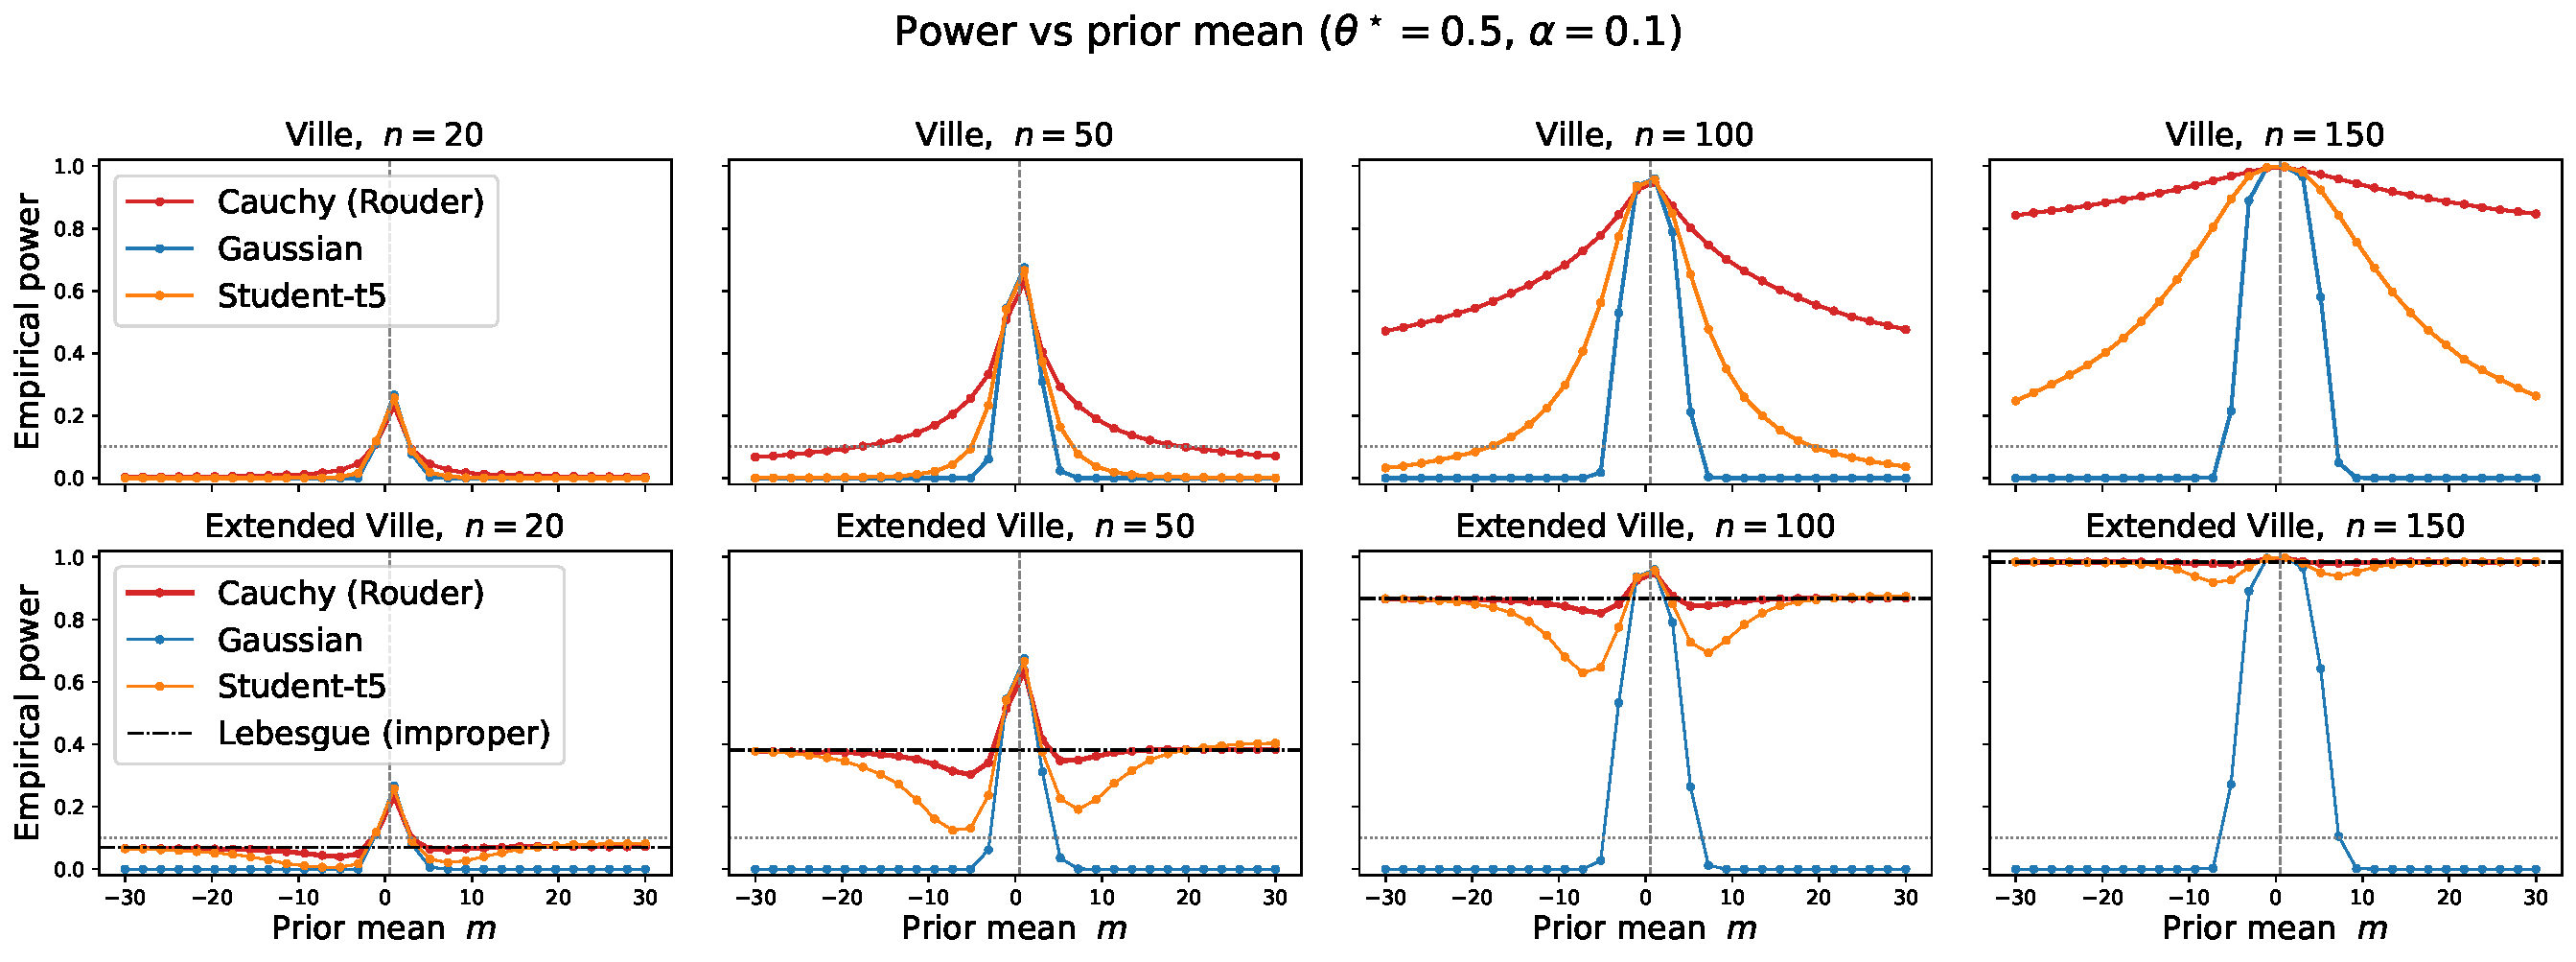
\includegraphics[width=\linewidth, height=0.4\linewidth]{images/power_vs_m_priors_shortened.pdf}
    \caption{Plot of Empirical power of the Ville (top row) and extended-Ville (bottom row) vs prior location parameter \(m\) for testing $H_0 : \theta = 0$ vs $H_1: \theta \neq 0$; true data parameter \(\theta^\star=0.5\), sample sizes \(n\in\{20,50,100,150\}\). Each panel uses \(B=10{,}000\) data replicates and \(B_{\mathrm{cal}}=100{,}000\) calibration replicates. The dashed vertical line marks the
    well-specified location \(m=\theta^\star\); the dotted horizontal
    line marks the level of significance \(\alpha=0.1\); the dash-dotted black line in the bottom row marks the non-informative Lebesgue extended-Ville baseline.}
    \label{fig:power_vs_m_priors}
\end{figure}

We illustrate the theory through a simulation study and visualise the empirical power vs prior location. Throughout we set \(\sigma=1\), so the data generated from $\mathcal{N}(0.5, 1)$ coincides with the standardised effect size \(\theta^\star = 0.5\). Let us now consider the anytime-valid test of \(H_0:\theta=0\) against \(H_1:\theta\neq0\) at fixed sample size \(n\) with level \(\alpha = 0.1\), and consider \(n\in\{20,50,100,150\}\). For each prior \(\pi\) and each location \(m\) on the grid \(\mathcal M\) on \([-30, 30]\), we draw \(B=10{,}000\) datasets
\(Y_{1:n}^{(b)}\stackrel{\mathrm{iid}}{\sim}\mathcal N(\theta^\star,1)\)
and report the empirical Ville and extended-Ville rejection rates,
\(\widehat{\mathrm{pow}}^{V}_{n,\alpha}(m)\) and
\(\widehat{\mathrm{pow}}^{eV}_{n,\alpha}(m)\), defined as the fraction
of replicates for which the corresponding \(p\)-variable falls at or
below \(\alpha\).

We compare the proper priors Cauchy (with the Rouder-JZS default scale $\frac{1}{\sqrt{2}} \approx 0.707$), Gaussian (with $\sigma = 1$) and Student-\(t\) (with degrees of freedom $5$ and scale $=1$); the improper Lebesgue prior of Section~\ref{subsec:improper-prior} serves as a non-informative baseline in the extended-Ville. The marginal likelihoods \(M_n^{\Pi_m}\) admit no closed form for these priors and are computed by adaptive Gauss-Kronrod quadrature in \(\theta\) \citep{piessens2012quadpack}, while the calibration functions
\(g_0^{(m)}\) are obtained by Monte Carlo under \(\Prob_0\) with
\(B_{\mathrm{cal}}=100{,}000\) replicates. Note that the law of \(M_2^{\Pi_m}(Y_{1:2})\) under \(\Prob_0\) depends on \(m\), so the calibration must be recomputed across the grid; however a single \(\Prob_0\)-sample of pairs \((Y_1^{(j)},Y_2^{(j)})\) suffices for the entire grid, since \(M_2^{\Pi_m}(Y_1^{(j)},Y_2^{(j)})\) can be evaluated for every \(m\in\mathcal M\) on the same Monte Carlo draws. The Lebesgue baseline uses the closed-form derived in Proposition~\ref{thm:Mn-Leb}, so it has no Monte Carlo error. Figure~\ref{fig:power_vs_m_priors} shows that both the Ville and the extended-Ville procedure attain their maximum power near the true effect \(\theta^\star=0.5\) and gradually decreases when the prior-data conflict increases. The Ville eventually drops to $0$ while the extended Ville reverts back to the Lebesgue baseline, making it robust against the prior-data conflict.



\subsection{Experiment on Real-Data}
\begin{figure}[h]
    \centering
    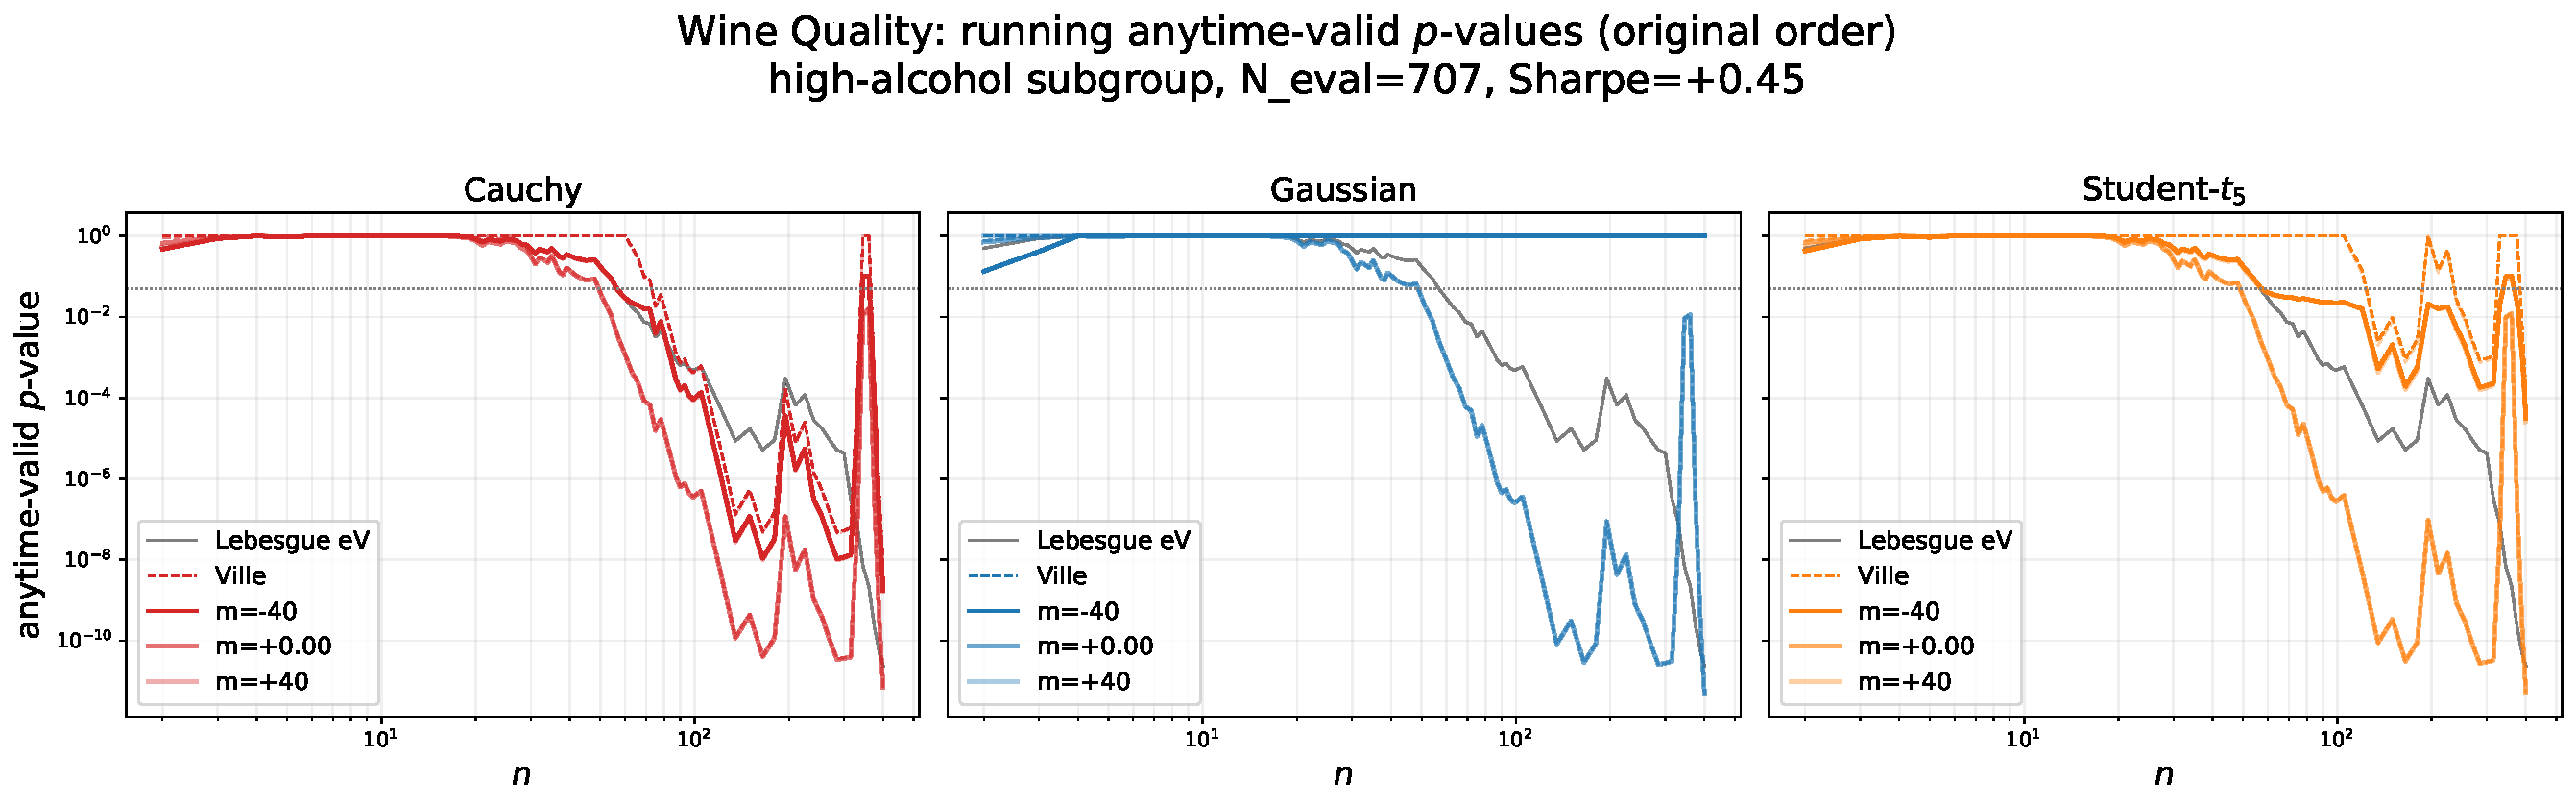
\includegraphics[width=\linewidth]{images/wine_pvalue_trajectory.pdf}
    \caption{Anytime-valid $p$-value trajectories for the Wine Quality dataset under five prior families. Solid lines represent the Extended Ville procedure, dashed lines the Ville procedure, and the thin black line the Lebesgue e-value baseline. Darker curves correspond to prior locations closer to the empirical data mean.}
    \label{fig:wine_pval_trajectory}
\end{figure}

We now turn from simulated data to a real dataset, where the effect is fixed by the data. We use the red-wine subset of the wine-quality data of \citet{Cortez2009}, which records a sensory quality score, on an integer scale, for each of $1{,}599$ wines together with their physicochemical properties. To obtain a one-sample problem with a genuine effect, we split the wines by alcohol content, which is among the strongest correlates of quality, and ask whether the above-median-alcohol wines differ in quality from the sample as a whole. Let $Y_i$ denote the quality score of high-alcohol wine $i$, centred at the overall mean, and let $\theta^\star = \mathbb{E}[Y_i]/\sqrt{\operatorname{Var}(Y_i)}$ be its standardised effect. We test $H_0:\theta^\star=0$ against a two-sided alternative, the scale-invariant problem of Section~\ref{subsec:improper-prior} with unknown variance. 

\begin{figure}[h]
    \centering
    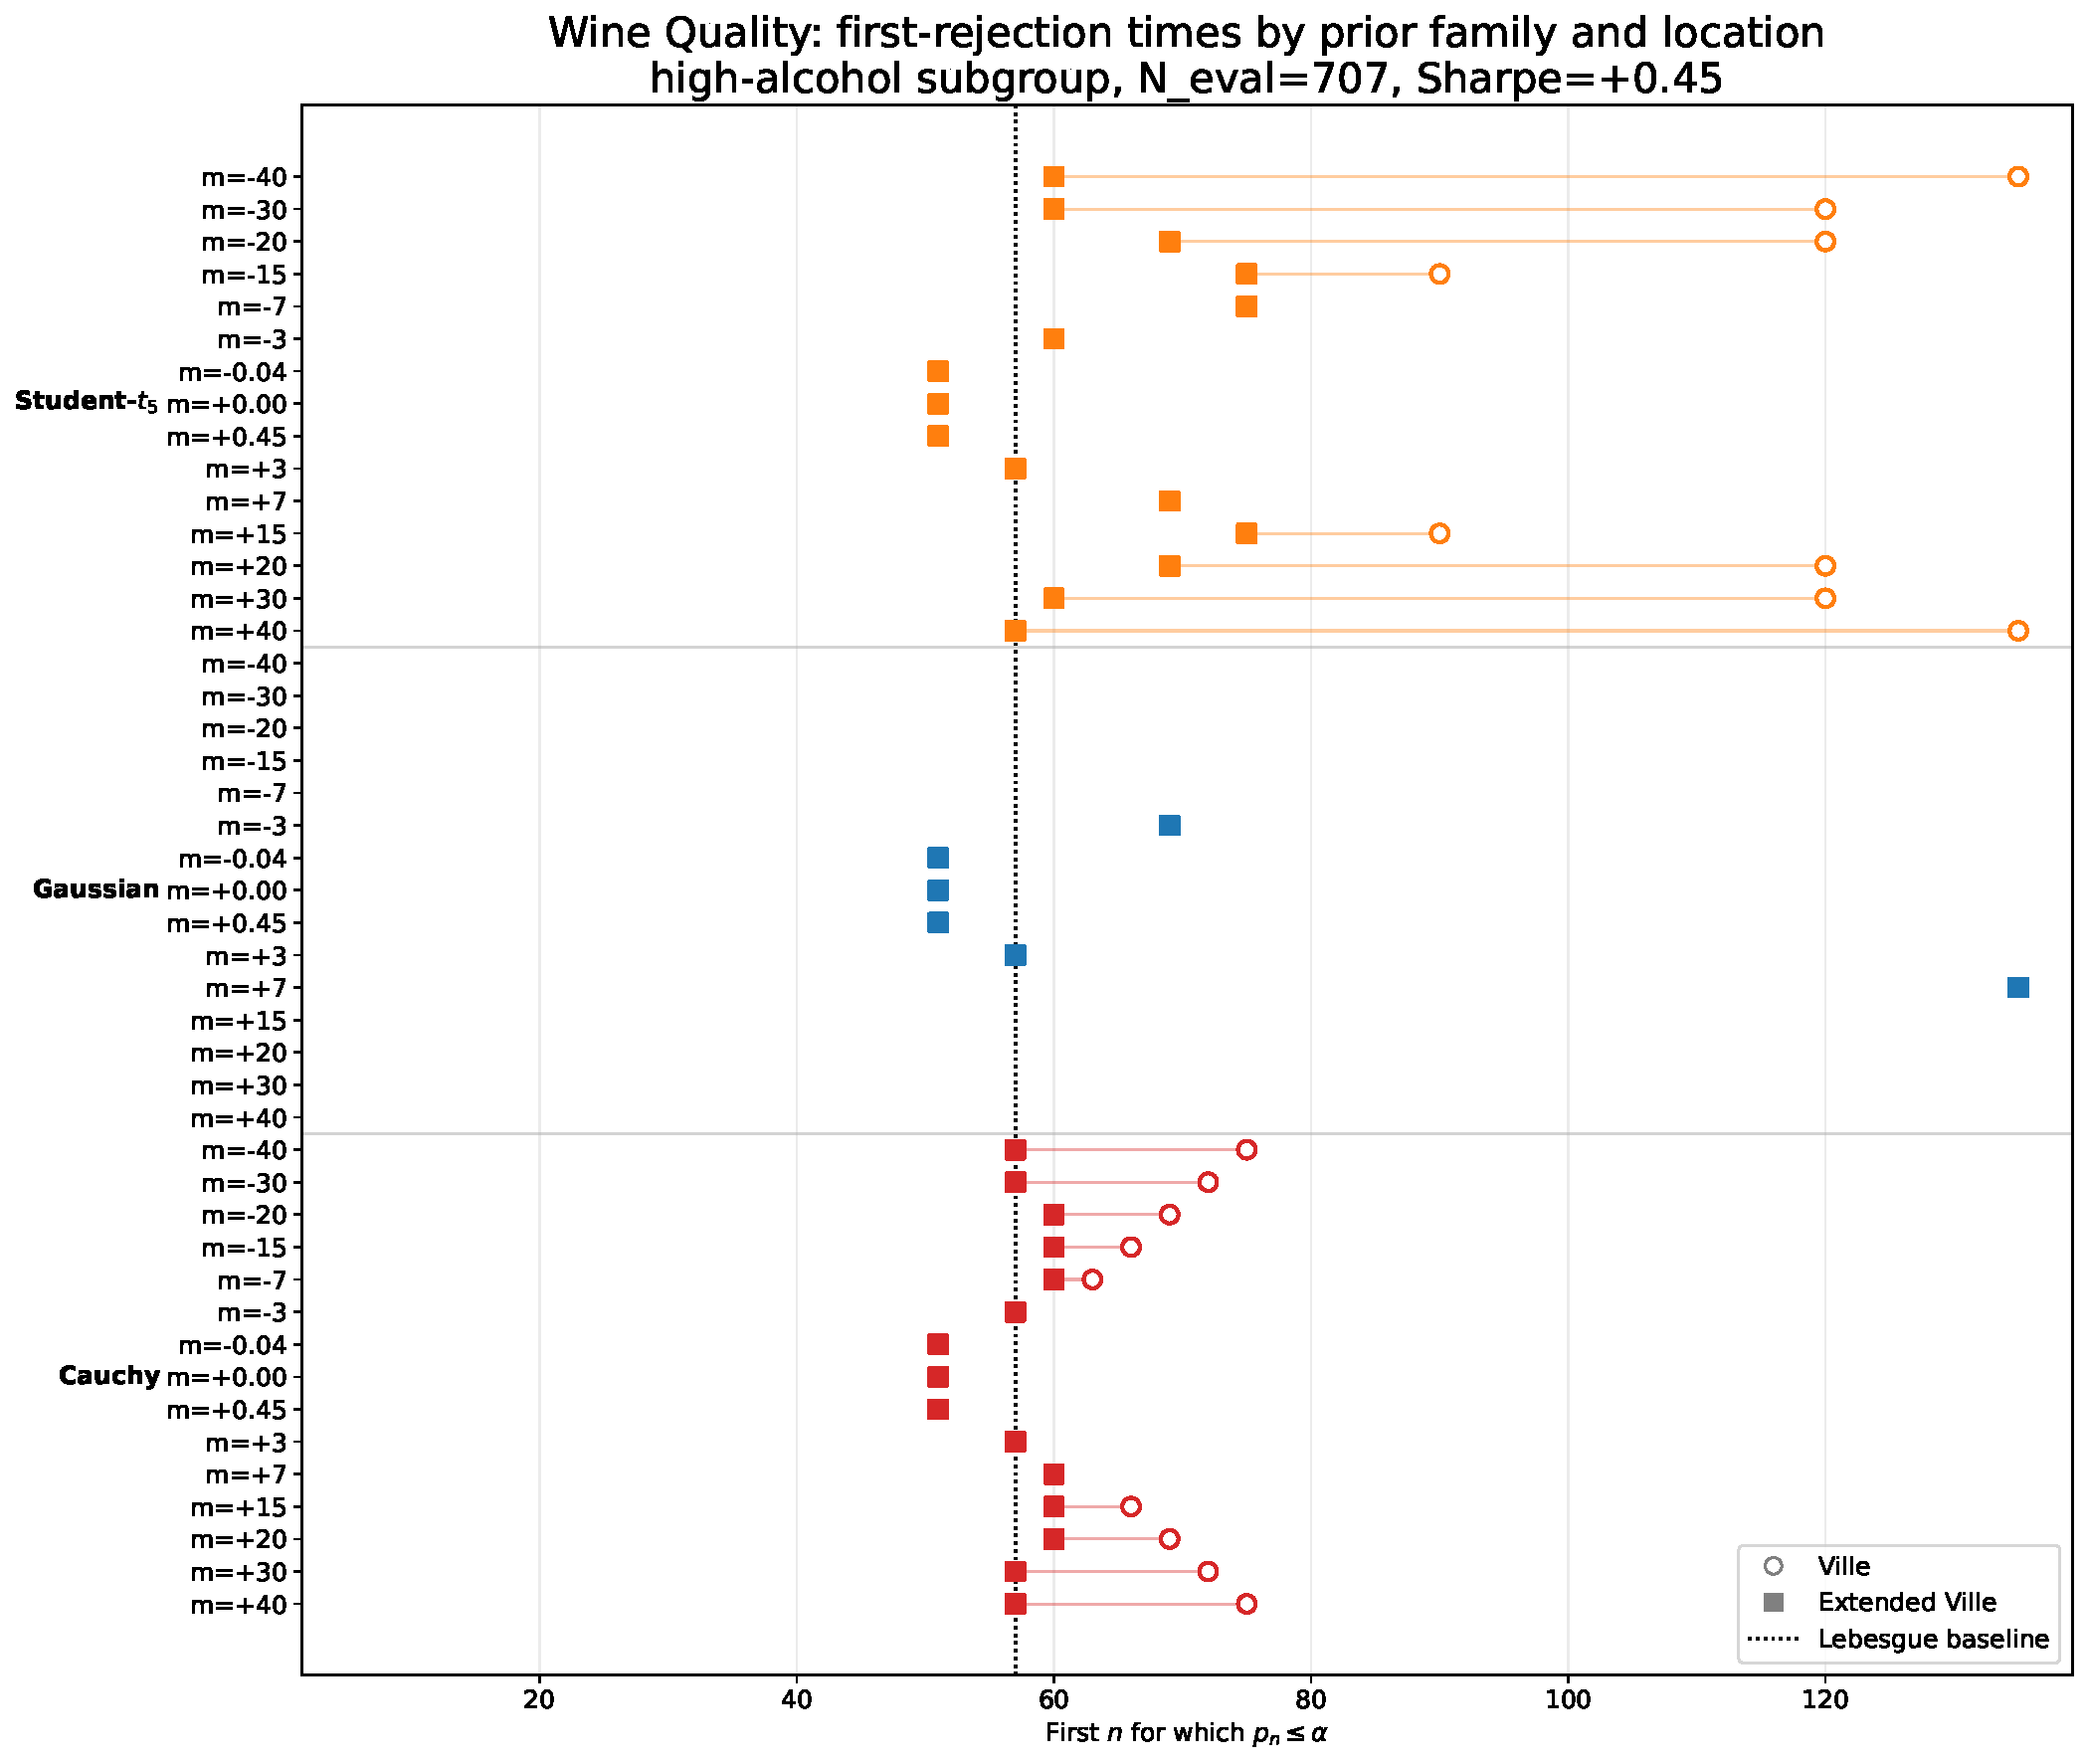
\includegraphics[width=\linewidth]{images/wine_first_rejection.pdf}
    \caption{First rejection time ($n$) at which $p_n \leq \alpha$ for the Wine Quality dataset, evaluated across multiple prior families and location parameters. Results are shown for the Ville (circles) and Extended Ville (squares) procedures, with the Lebesgue baseline indicated by the dotted vertical line.}
    \label{fig:wine_first_rej}
\end{figure}

Rather than fix the prior location in advance, we estimate it from a pilot sample. We hold out the first $N_{\mathrm{cal}}=50$ observations out of the $757$ of the subgroup as a pilot set $\mathcal C$ and take the prior location to be its sample Sharpe ratio, $\widehat m_{\mathrm{EB}}=\bar Y_{\mathcal C}/S_{\mathcal C}$. The remaining $N_{\mathrm{eval}}=707$ observations form the sequence on which the anytime-valid procedures are run with the standardised effect is $\widehat\theta_N\approx 0.45$. We take $\alpha=0.05$ throughout. We use the same priors and grid of locations $m$ as in Section~\ref{sec:sim1}, now ranging from the pilot estimate $\widehat m_{\mathrm{EB}}$ out to severe prior-data conflict at $|m|=40$, with the improper Lebesgue prior of Section~\ref{subsec:improper-prior} as the non-informative baseline.

Figures~\ref{fig:wine_pval_trajectory} and~\ref{fig:wine_first_rej} exhibit the same qualitative behaviour as in the simulations. The Extended Ville procedure is uniformly at least as efficient as the Ville procedure, with the advantage becoming most pronounced when the prior location is substantially misspecified.








\begin{appendices}

\section{Proofs}
\label{sec:proofs}



\subsection{Proof of Proposition \ref{thm:Mn-Leb}}

This is already in Wang and Ramdas, just included here for completeness.\fc{todo}


\subsection{Proof of Theorem \ref{thm:recovery}}



\begin{proof}
We recall that
$$
h_{n}(\theta,u)=e^{-n\theta^2/2 }A_n(u \theta ).
$$
Write $M_{n,m}(u)=\int h_n(\theta,u)\Pi(\dd\theta)$ and $M_{n,m}^\Leb(u)=\int h_n(\theta,u)\dd\theta$. 

\emph{Step 1 (ratio convergence).}  Fix $R>0$ and split
\[
  \frac{M_{n,m}(u)}{a_m}
  \;=\;\underbrace{\int_{|\theta|\leq R}}_{=:I_1(R,m)}
   +\underbrace{\int_{R<|\theta|\leq m/2}}_{=:I_2(R,m)}
   +\underbrace{\int_{|\theta|>m/2}}_{=:I_3(m)}\;
   h_{n}(\theta,u)\,\frac{\pi(\theta-m)}{a_m}\,\dd\theta.
\]
We have, for any $\theta$,
$$
\pi(\theta-m)\sim a_m \sim m^{-\beta}L_-(m)
$$
as $m\to\infty$. By the uniform convergence theorem for regularly varying functions
\citep[Theorem~1.2.1]{Bingham1987}, 
$$
\sup_{|\theta|\leq R}|\pi(\theta-m)/a_m-1|\to 0
$$
as $m\to\infty$, so 
$$
I_1(R,m)\to\int_{|\theta|\leq R}h_{n}(\theta,u)\,\dd\theta.
$$
For $I_2$, on $|\theta|\leq m/2$ we have $|\theta-m|\in[m/2,\,3m/2]$, so
regular variation yields a constant $C_\star<\infty$ (independent of $R$ and of
$m$ for all large $m$) such that $\pi(\theta-m)/a_m\leq C_\star$; hence
$$
I_2(R,m)\leq C_\star\int_{|\theta|>R}h_{n}(\theta,u)\,\dd\theta,
$$ which vanishes
as $R\to\infty$. For $I_3$, using the fact that $\pi$ is a proper prior
(i.e.\ $\int_\mathbb{R}\pi=1$),
\[
I_3(m)\;=\;\int_{|\theta|>m/2}h_{n}(\theta,u)\,\frac{\pi(\theta-m)}{a_m}\,\dd\theta
   \;\leq\; a_m^{-1}\sup_{|\theta|>m/2}h_{n}(\theta,u),
\]
the supremum is exponentially small in $m$ by \eqref{eq:hu-env}, while $a_m$ is
only polynomially small, so $I_3(m)\to 0$.

Combining these three bounds, for each fixed $R>0$,
\begin{align*}
   \int_{|\theta|\leq R}h_{n}(\theta,u)\,\dd\theta
   \;\leq\; \liminf_{m\to\infty}\frac{M_{n,m}(u)}{a_m}
   &\;\leq\; \limsup_{m\to\infty}\frac{M_{n,m}(u)}{a_m}\\
   & \;\leq\; \int_{|\theta|\leq R}h_{n}(\theta,u)\,\dd\theta
   \;+\; C_\star\!\int_{|\theta|>R}h_{n}(\theta,u)\,\dd\theta.
\end{align*}
Sending $R\to\infty$ and using $\int_\mathbb{R} h_{n}(\theta,u)\,\dd\theta
= M_n^{\Leb}(u)$ gives \eqref{eq:Mnm-asymp}.

\emph{Step 2 (calibration convergence).}
Since \(|U_2|<\sqrt 2\) almost surely under \(\Prob_0\), Step~1 applied with \(n=2\) gives
\(M_{2,m}(U_2)/a_m\to M_2^{\Leb}(U_2)\) almost surely. Since \(0\leq\min(M_{2,m}(U_2)/(a_m c),1)\leq 1\), bounded convergence yields
\[
  g_m(a_m c)
  \;=\;\E_0\!\Bigl[\min\!\Bigl(\tfrac{M_{2,m}(U_2)}{a_mc},1\Bigr)\Bigr]
  \;\longrightarrow\;
  \E_0\!\Bigl[\min\!\Bigl(\tfrac{M_2^{\Leb}(U_2)}{c},1\Bigr)\Bigr]
  \;=\;g_{\Leb}(c),
\]
proving \eqref{eq:gm-asymp}.

\emph{Step 3 (composition).}
Set \(c_m:=M_{n,m}(u_n)/a_m\) and \(c:=M_n^{\Leb}(u_n)\); by Step~1 \(c_m\to c\). Each \(g_m\) is decreasing, so for any \(\varepsilon\in(0,c)\) and \(m\) large, \(g_m(a_m(c+\varepsilon))\leq g_m(a_m c_m)\leq g_m(a_m(c-\varepsilon))\). Taking \(\liminf\) and \(\limsup\) using Step~2 and letting \(\varepsilon\downarrow 0\) yields \eqref{eq:p-asymp}.
\end{proof}




\section{Secondary lemmas}
\label{sec:secondarylemmas}

\begin{lemma}\label{lemma:hthetabound}
For $n\geq 2$, $|u|<\sqrt{n}$, $\theta\in\bbR$, let 
  \begin{equation}
\label{eq:hthetadef2}
  h_{n}(\theta,u)
  =
  e^{-n\theta^2/2}
  A_n\bigl(\theta u\bigr),
\end{equation}
where $A_n$ is the MGF of $\chi_n$.  Then, for any $u^2<\eta<n$, 
\begin{equation}
h_{n}(\theta,u)\leq \exp\left(-\frac{(n-\eta)\theta^2}{2}\right)\left(1-\frac{u^2}{\eta}\right)^{-n/2}.
\label{eq:hu-env}
\end{equation}
Thus, there are constants $C_{n,u}$,$\kappa_{n,u}>0$ such that 
$$
0\leq h_{n}(\theta,u)\leq C_{n,u}e^{-\kappa_{n,u}\theta^2}.
$$
\end{lemma}

\begin{proof}
\fc{TODO}
\end{proof}


\begin{lemma}\label{sec:asymp_An}
For $R_n\sim\chi_n$, let
\[
A_n(z)=\mathbb E[e^{z R_n}]=\frac{1}{\Gamma(n/2)}\int_0^\infty y^{n/2-1}\exp(-y+z\sqrt{2y})dy.
\]
Then
$$A_n(z) \sim \frac{2^{1-n/2}}{\Gamma(n/2)} \sqrt{2\pi} z^{n-1} e^{z^2/2}$$ as $z \longrightarrow \infty$.
\end{lemma}











\begin{proof}
Substituting \(r=\sqrt{2y}\), so that \(y=r^2/2\) and
\(dy=r\,dr\), and completing the square, we obtain
\[
A_n(z)
=
\frac{2^{1-n/2}}{\Gamma(n/2)}
e^{z^2/2}
\int_0^\infty
r^{n-1}e^{-(r-z)^2/2}\,dr.
\]
Setting \(u=r-z\) gives
\[
\int_0^\infty
r^{n-1}e^{-(r-z)^2/2}\,dr
=
z^{n-1}
\int_{-z}^\infty
\left(1+\frac{u}{z}\right)^{n-1}
e^{-u^2/2}\,du.
\]
For each fixed \(u\in\mathbb{R}\),
\[
\left(1+\frac{u}{z}\right)^{n-1}
\mathbf{1}_{\{u>-z\}}
\longrightarrow 1
\qquad \text{as } z\to\infty.
\]
Moreover, for \(z\geq 1\), the integrand is bounded by
\[
(1+|u|)^{n-1}e^{-u^2/2},
\]
which is integrable on \(\mathbb{R}\). Therefore, by the dominated
convergence theorem,
\[
\int_{-z}^\infty
\left(1+\frac{u}{z}\right)^{n-1}
e^{-u^2/2}\,du
\longrightarrow
\int_{-\infty}^\infty e^{-u^2/2}\,du
=
\sqrt{2\pi}.
\]
Consequently,
\[
A_n(z)
\sim
\frac{2^{1-n/2}}{\Gamma(n/2)}
\sqrt{2\pi}\,
z^{n-1}e^{z^2/2},
\qquad z\to\infty.
\]
\end{proof}


\end{appendices}

\section*{Competing interests}
%No competing interest is declared.

\section*{Author contributions statement}

%Must include all authors, identified by initials, for example:
%S.R. and D.A. conceived the experiment(s),  S.R. conducted the experiment(s), S.R. and D.A. analysed the results.  S.R. and D.A. wrote and reviewed the manuscript.


\section*{Copyright Licence}
For the purpose of open access, the authors have applied a CC BY public copyright licence to any author accepted manuscript arising from this submission.


\section*{Acknowledgments}
%The authors thank the anonymous reviewers for their valuable suggestions. This work is supported in part by funds from the National Science Foundation (NSF: \# 1636933 and \# 1920920).


\bibliographystyle{abbrvnat}
\bibliography{robustttest}


\end{document}
